\chapter{Interpolación y ajuste de funciones}\label{interpolacion}

\epigraph{Digo que ya tú sabes que la humildad es la basa y fundamento de todas las virtudes, y que sin ella no hay alguna que lo sea. Ella allana inconvenientes, vence dificultades, y es un medio que siempre a gloriosos fines nos conduce; de los enemigos hace amigos, templa la cólera de los airados y menoscaba la arrogancia de los soberbios; es madre de la modestia y hermana de la templanza; en fin, con ella no pueden atravesar triunfo que les sea de provecho los vicios, porque en su blandura y mansedumbre se embotan y despuntan las flechas de los pecados.}{El coloquio de los perros. Miguel de Cervantes}


\begin{paracol}{2}
En este capítulo vamos a estudiar distintos métodos de aproximación polinómica. En términos generales el problema consiste en sustituir una función $f(x)$ por un polinomio,
\end{paracol}
\begin{equation*}
f(x)\approx p(x)=a_0+a_1\cdot x+a_2\cdot x^2+a_3\cdot x^3+\cdots +a_n \cdot x^n
\end{equation*}
\begin{paracol}{2}
Para obtener la aproximación podemos partir de la ecuación que define $f(x)$,  por ejemplo la función error,
\end{paracol}
\begin{equation*}
erf(x)=\frac{2}{\sqrt{\pi}}\int_0^x e^{-t^2}dt
\end{equation*}
\begin{paracol}{2}
O bien, puede suceder que solo conozcamos algunos valores de la función, por ejemplo a través de una tabla de datos,
\end{paracol}
\begin{table}[h]
\caption{$f(x)=erf(x)$}
\centering
\begin{tabular}{c|c}
$x$&$f(x)$\\ 
\hline
$0.0$& $0.0000$\\
$0.1$&$0.1125$\\
$0.2$&$0.2227$\\
$0.3$&$0.3286$\\
$0.4$&$0.4284$\\
$0.5$&$0.5205$\\
\end{tabular}
\label{tpuntos2}
\end{table}

\begin{paracol}{2}
La aproximación de una función por un polinomio, tiene ventajas e inconvenientes. 

Probablemente la principal ventaja, desde el punto de vista del cómputo, es que un polinomio es fácil de evaluar  mediante un ordenador ya que solo involucra operaciones aritméticas sencillas. Además, los polinomios son fáciles de derivar e integrar, dando lugar a otros polinomios.

En cuanto a los inconvenientes hay que citar el crecimiento hacia infinito o menos infinito de cualquier polinomio para valores de la variable independiente alejados del origen. Esto puede dar lugar en algunos casos a errores de redondeo difíciles de manejar, haciendo muy difícil la aproximación para funciones no crecientes.

Vamos a estudiar tres métodos distintos; en primer lugar veremos la aproximación mediante el polinomio de Taylor, útil para aproximar una función en las inmediaciones de un punto. A continuación,  veremos la interpolación polinómica y, por último, estudiaremos el ajuste polinómico por mínimos cuadrados.

El uso de uno u otro de estos métodos esta asociado a la información disponible sobre la función que se desea aproximar y al uso que se pretenda hacer de la aproximación realizada.


\section{El polinomio de Taylor.}\index{Polinomio de Taylor}

Supongamos una función infinitamente derivable en un entorno de un punto $x_0$. Su expansión en serie de Taylor se define como,
\end{paracol}
\begin{equation*}
f(x)=f(x_0)+f'(x_0)\cdot (x-x_0)+\frac{1}{2} f''(x_0)\cdot (x-x_0)^2+\cdots + \frac{1}{n!}f^{(n)}(x_0)\cdot (x-x_0)^n+ \frac{1}{(n+1)!}f^{(n+1)}(z)\cdot (x-x_0)^{n+1}
\end{equation*}

\begin{paracol}{2}
Donde $z$ es un punto sin determinar situado entre $x$  y $x_0$.   Si eliminamos el último término, la función puede aproximarse por un polinomio de grado $n$								
\end{paracol}
\begin{equation*}
f(x)\approx f(x_0)+f'(x_0)\cdot (x-x_0)+\frac{1}{2}f''(x_0)\cdot (x-x_0)^2+\cdots + \frac{1}{n!}f^{(n)}(x_0)\cdot (x-x_0)^n
\end{equation*}
\begin{paracol}{2}
El error cometido al aproximar una función por un polinomio de Taylor de grado $n$, viene dado por el término,
\index{Polinomio de Taylor! Error de la aproximación}
\end{paracol}
\begin{equation*}
e(x)=\lvert f(x) -p(x)\rvert=\left\lvert\frac{1}{(n+1)!} f^{(n+1)}(z)\cdot (x-x_0)^{n+1}\right\rvert
\end{equation*}
\begin{paracol}{2}
Es fácil deducir de la ecuación que el error disminuye con el grado del polinomio empleado y aumenta con la distancia entre $x$ y $x_0$. Además cuanto más suave es la función (derivadas pequeñas) mejor es la aproximación.

Por ejemplo para la función exponencial, el polinomio de Taylor de orden $n$ desarrollado en torno al punto $x_0=0$ es, \index{Polinomio de Taylor! Serie de la función exponencial}
\end{paracol}
\begin{equation*}
e^x\approx 1+x+\frac{1}{2}x^2+\cdots+\frac{1}{n!}x^n=\sum_{i=0}^n\frac{1}{i!}x^i
\end{equation*}
\begin{paracol}{2}
y el del logaritmo natural, desarrollado en torno al punto $x_0=1$, \index{Polinomio de Taylor! Serie del logaritmo natural}
\end{paracol}
\begin{equation*}
\log(x)\approx (x-1)-\frac{1}{2}(x-1)^2+\cdots+\frac{(-1)^{n+1}}{n}(x-1)^n=\sum_{i=1}^n\frac{(-1)^{i+1}}{i}(x-1)^i
\end{equation*}
\begin{paracol}{2}
La existencia de un término general para los desarrollos de Taylor de muchas funciones elementales lo hace particularmente atractivo para aproximar funciones mediante un ordenador. Así por ejemplo, la siguiente función de Matlab, aproxima el valor del logaritmo natural en un punto, empleando un polinomio de Taylor del grado que se desee,
\end{paracol}

\inputminted[
frame=lines,
framesep=2mm,
baselinestretch=1.2,
%bgcolor=LightGray,
label=determinante.py,
fontsize=\footnotesize,
linenos
]{python}{./codigos/Algebra/codigo_abierto/determinante.py}


%\begin{lstlisting}
%function y=taylorln(x,n)
% Esta función aproxima el valor del logaritmo natural de un numero
% empleando para ello un polinomio de Taylor de grado n desarrollado en 
% torno a x=1. Las variables de entrada son: x, valor para el que se desea 
% calcular el logaritmo. n Grado del polinomio que se empleará en el 
% cálculo. La variable de salida y es el logaritmo de x. (nota si x
% es un vector, calculará el logaritmo para todos los puntos del vector)

% iniciliazamos la variable de salida y
%y=0;

% construimos un búcle para ir añadiendo términos al desarrollo
%for i=1:n
%    y=y+(-1)^(i+1)*(x-1).^i/i;
%end
%\end{lstlisting}
\begin{paracol}{2}
La aproximación funciona razonablemente bien para puntos comprendidos en el intervalo $0<x<2$. La figura \ref{fig:ln} muestra los resultados obtenidos en dicho intervalo para polinomios de Taylor del logaritmo natural de grados 2, 5, 10 20. La linea continua azul representa el valor del logaritmo obtenido con la función de Matlab \texttt{log}.
\end{paracol}
\begin{figure}[h]
\centering
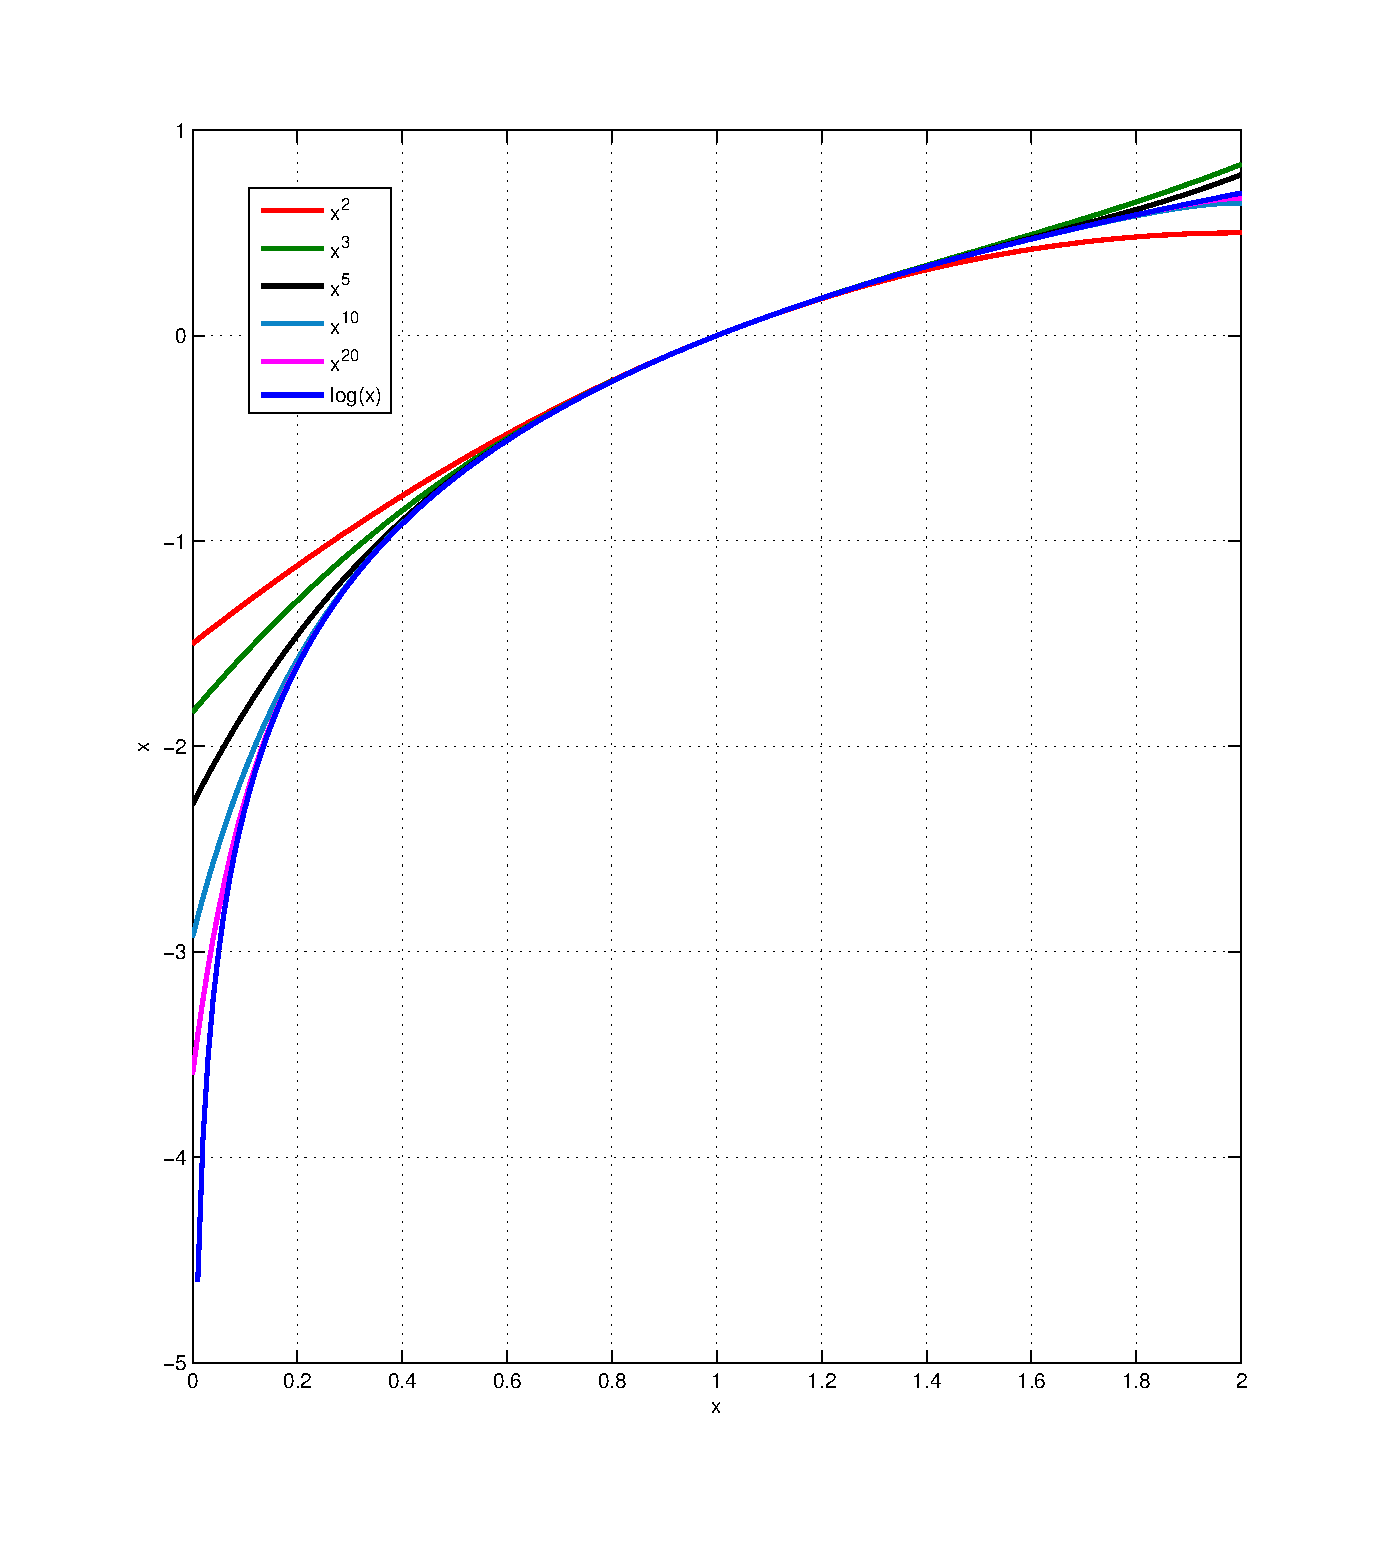
\includegraphics[width=12cm]{ln.eps}
\caption{Comparación entre resultados obtenidos para polinomios de Taylor del logaritmo natural. (grados 2, 3, 5, 10, 20)}
\label{fig:ln}
\end{figure}
\begin{paracol}{2}
\index{Polinomio de Taylor! Series de las funciones seno y coseno}
Las funciones $\sin(x)$ y $\cos(x)$, son también simples de aproximar mediante polinomios de Taylor. Si desarrollamos en torno a $x_0=0$, la serie del coseno solo tendrá potencias pares mientras que la del seno solo tendrá potencias impares,
\end{paracol}
\begin{align*}
\cos(x)&\approx \sum_{i=0}^n \frac{(-1)^i}{(2i)!}x^{2i}\\
\sin(x)&\approx \sum_{i=0}^n \frac{(-1)^i}{(2i+1)!}x^{2i+1}
\end{align*}

\begin{figure}[h]
\centering
\subfigure[$\cos(x)$, polinomios 2, 4, 6 y 8 grados  \label{fig:cos}]{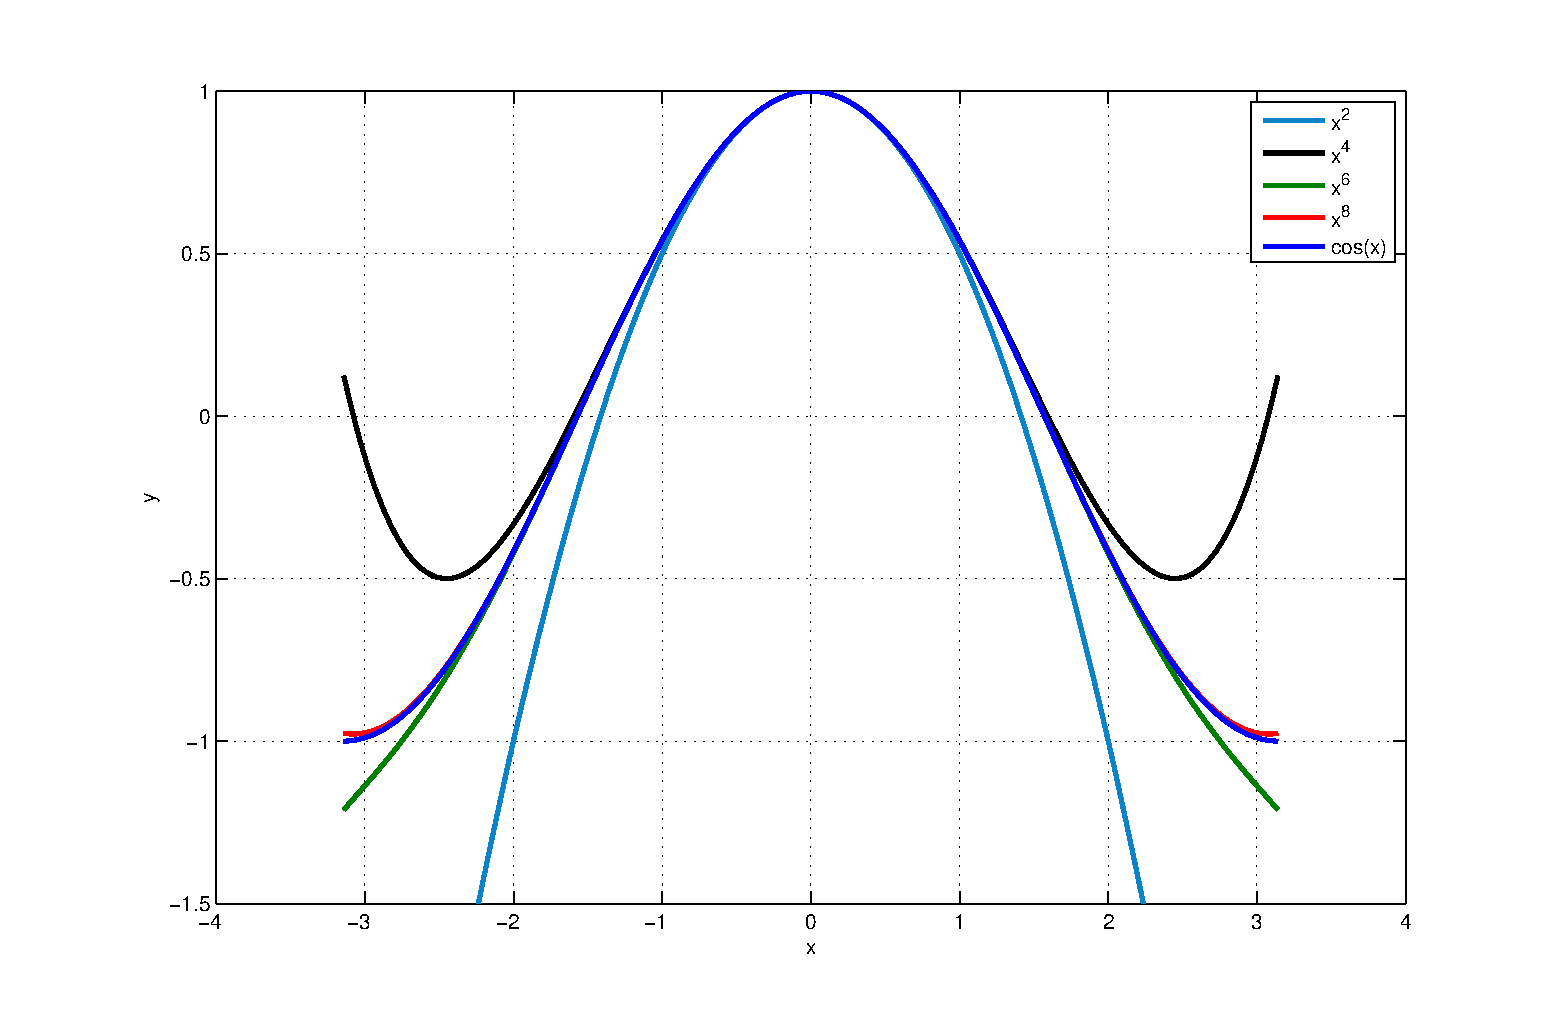
\includegraphics[width=10.5cm]{cos.eps}} \qquad 
\subfigure[$\sin(x)$, polinomios  3, 5, 7 y 9  grados \label{fig:sin}]{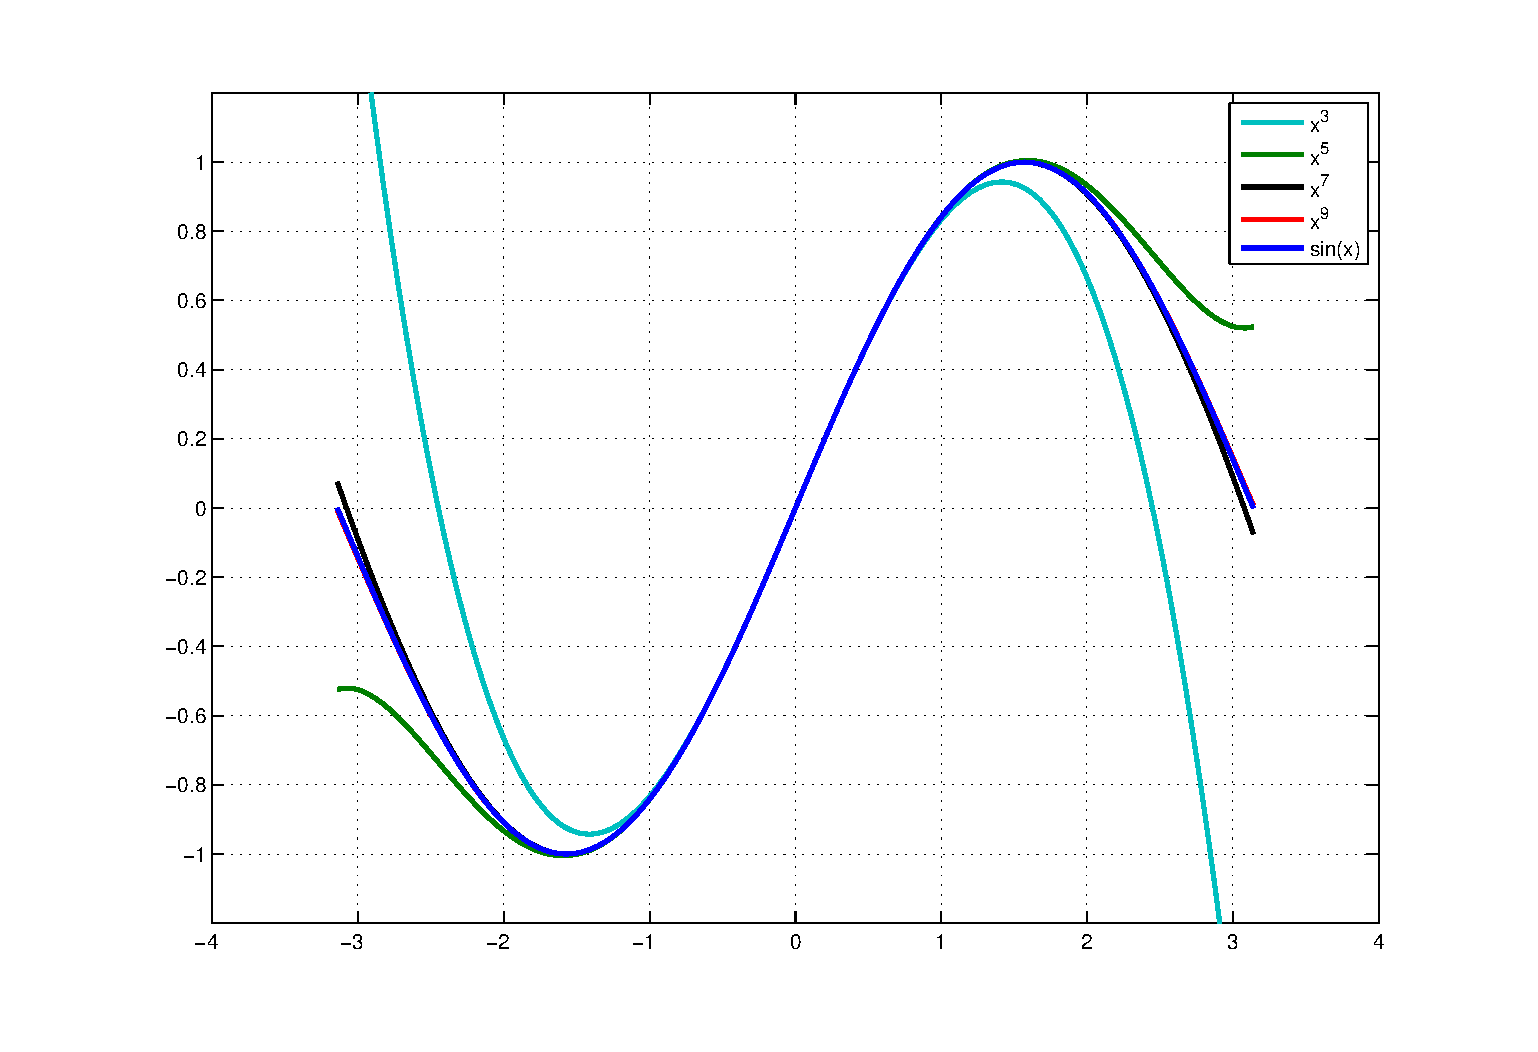
\includegraphics[width=10.5cm]{sin.eps}}\\
\caption{Polynomios de Taylor para las funciones coseno y seno  }
\end{figure}
\begin{paracol}{2}
En las figuras \ref{fig:cos} y \ref{fig:sin} Se muestran las aproximaciones mediante polinomios de Taylor de las funciones coseno y seno. Para el coseno se han empleado polinomios hasta grado 8 y para el seno hasta grado 9. En ambos casos se dan los resultados correspondientes a un periodo $(-\pi, \pi)$. Si se comparan los resultados con las funciones \texttt{cos} y \texttt{sin}, suministradas por Matlab, puede observarse que la aproximación es bastante buena para los polinomios de mayor grado empleados en cada caso.

\section{Interpolación polinómica.}

Se entiende por interpolación el proceso por el cual, dado un conjunto de pares de puntos $(x_0,y_0),(x_1,y_1),\cdots (x_n,y_n)$ se obtiene una función $f(x)$, tal que, $y_i=f(x_i)$, para cada par de puntos $(x_i,y_i)$ del conjunto. Si, en particular, la función empleada es un polinomio $f(x)\equiv p(x)$, entonces se trata de interpolación polinómica. \index{Interpolación! Polinómica}

\paragraph{Teorema de unicidad.} Dado un conjunto \index{Interpolación! Teorema de unicidad}  $(x_0,y_0),(x_1,y_1),\cdots (x_n,y_n)$ de $n+1$ pares de puntos, tales que todos los valores $x_i$ de dicho conjuntos son diferentes entre sí, solo existe un polinomio $p(x)$ de grado $n$, tal que $y_i=p(x_i)$ para todos los pares de puntos del conjunto.

Si tratamos de interpolar los puntos con un polinomio de grado menor que $n$, es posible que no encontremos ninguno que pase por todos los puntos. Si, por el contrario empleamos un polinomio de grado mayor que $n$, nos encontramos con que no es único. Por último si el polinomio empleado es de grado $n$, entonces será siempre el mismo con independencia del método que empleemos para construirlo.

\subsection{La matriz de Vandermonde} \index{Matriz de Vandermonde}
Supongamos que tenemos un conjunto de pares de puntos $\mathcal{A}$, 
\end{paracol}
\begin{table}[h]
%\caption{$f(x)=erf(x)$}
\centering
\begin{tabular}{c|c}
$x$&$f(x)$\\ 
\hline
$x_0$& $y_0$\\
$x_1$&$y_1$\\
$x_2$&$y_2$\\
$\vdots$&$\vdots$\\
$x_n$&$y_n$
\end{tabular}
\label{tpuntos3}
\end{table}
\begin{paracol}{2}
Para que un polinomio de orden $n$,
\end{paracol}
\begin{equation*}
p(x)=a_0+a_1x+a_2x^2+\cdots+a_nx^n
\end{equation*}
\begin{paracol}{2}
pase por todos los pares de $\mathcal{A}$ debe cumplir,
\end{paracol}
\begin{equation*}
y_i=a_0+a_1x_i+a_2x_i^2+\cdots+a_nx_i^n, \ \forall (x_i,y_i) \in \mathcal{A}
\end{equation*}
\begin{paracol}{2}
Es decir, obtendríamos un sistema de $n$ ecuaciones lineales, una para cada par de valores, en la que las incógnitas son precisamente los $n$ coeficientes $a_i$ del polinomio.

Por ejemplo para los puntos,
\end{paracol}
\begin{table}[h]
%\caption{$f(x)=erf(x)$}
\centering 
\begin{tabular}{c|c}
$x$&$f(x)$\\ 
\hline
$1$&$\ 2$\\
$2$&$ \ 1$\\
$3$&$-2$
\end{tabular}
\label{tpuntos4}
\end{table}
\begin{paracol}{2}
Obtendríamos,
\end{paracol}
\begin{align*}
a_0+a_1\cdot 1+ a_2\cdot 1^2&=2\\
a_0+a_1\cdot 2+ a_2\cdot 2^2&=1\\
a_0+a_1\cdot 3+ a_2\cdot 3^2&=-2
\end{align*}
\begin{paracol}{2}
que podríamos expresar en forma matricial como,
\end{paracol}

\begin{equation*}
\begin{pmatrix}
1&1&1^2\\
1&2&2^2\\
1&3&3^2
\end{pmatrix}\cdot \begin{pmatrix}
a_0\\
a_1\\
a_2
\end{pmatrix}=\begin{pmatrix}
2\\
1\\
-2
\end{pmatrix}
\end{equation*}
\begin{paracol}{2}
Y en general, para $n$ pares de datos,
\end{paracol}
\begin{equation*}
\begin{pmatrix}
1&x_0&x_0^2&\cdots &x_0^n\\
1&x_1&x_1^2&\cdots &x_1^n\\
\vdots&\vdots&\vdots&\ddots&\vdots\\
1&x_n&x_n^2&\cdots &x_n^n
\end{pmatrix}\cdot \begin{pmatrix}
a_0\\
a_1\\
\vdots\\
a_n

\end{pmatrix}=\begin{pmatrix}
y_0\\
y_1\\
\vdots\\
y_n
\end{pmatrix}
\end{equation*}
\begin{paracol}{2}
La matriz de coeficientes del sistema resultante recibe el nombre de matriz de Vandermonde. Está formada por la $n$ primeras potencias de cada uno de los valores de la variable independiente, colocados por filas. Es evidente que cuanto mayor es el número de datos, mayor tenderá a ser la diferencia de tamaño entre los elementos de cada fila. Por ello, en la mayoría de los casos, resulta ser una matriz mal condicionada para resolver el sistema numéricamente. En la práctica, para obtener el polinomio interpolador, se emplean otros métodos alternativos,

\subsection{El polinomio interpolador de Lagrange.} \label{sec:lagranje}\index{Interpolación! Polinomio de Lagrange} \index{Polinomio de Lagrange}

A partir de los valores $x_0, x_1,\cdots, x_n$, se construye el siguiente conjunto de $n+1$ polinomios de grado $n$
\end{paracol}
\begin{equation*}
l_j(x)=\prod_{\substack{k=0\\
k\neq j}}^n\frac{x-x_k}{x_j-x_k}=\frac{(x-x_0)(x-x_1)\cdots(x-x_{j-1})(x-x_{j+1})\cdots(x-x_n)}{(x_j-x_0)(x_j-x_1)\cdots(x_j-x_{j-1})(x_j-x_{j+1})\cdots(x_j-x_n)}
\end{equation*}
\begin{paracol}{2}
Los polinomios así definidos cumplen una interesante propiedad en  relación con los valores $x_0, x_1,\cdots, x_n$, empleados para construirlos,
\end{paracol}
\begin{equation*}
l_j(x_i)= \left\{ 
\begin{aligned}
1,\ i=j\\
0,\ i\neq j
\end{aligned}
\right.
\end{equation*}
\begin{paracol}{2}
A partir de estos polinomios podemos construir ahora el siguiente polinomio de interpolación empleando las imágenes $y_0,y_1\cdots, y_n$ correspondientes a los valores $x_0, x_1,\cdots, x_n$,
\end{paracol}
\begin{equation*}
p(x)=\sum_{j=0}^n l_j(x)\cdot y_j
\end{equation*}
\begin{paracol}{2}
Efectivamente, es fácil comprobar que, tal y como se ha construido, este polinomio pasa por los pares de puntos $x_i,y_i$, puesto que $p(x_i)=y_i$.

El siguiente código de Matlab calcula el valor en un punto x cualquiera del polinomio de interpolación de Lagrange construido a partir un conjunto de puntos $\mathcal{A}\equiv \{(x_i,y_i)\}$ . 
\end{paracol}
%\begin{lstlisting}
%function y1=Lagrange(x,y,x1)
% este programa obtiene el valor interpolado y1 correspondiente al valor x1
% empleando el polinomio interpolador de Lagrange de grado n, obtenido a 
% partir de los vectores x e y (de longitud n)

% obtenemos el tamaño del conjunto de datos,

%n=length(x);
% inicializamos la variable de salida
%y1=0;
% construimos el valor a partir de los polinomios de Lagrange,
%for j=1:n
    % inicializamos el polinomio de Lagrange correspondiente al dato i
%    lj=1;
    % y lo calculamos...
%    for i=1:j-1
%       lj=lj*(x1-x(i))/(x(j)-x(i));
%    end
%    for i=j+1:n
%       lj=lj*(x1-x(i))/(x(j)-x(i));
%    end 
    
    % sumamos la contribución del polinomio de Lagrange lj
%    y1=y1+lj*y(j);
%end
%\end{lstlisting}
\begin{paracol}{2}
\section{Diferencias divididas.}\label{sec:difdiv} \index{Interpolación! Diferencias Divididas} \index{Diferencias Divididas}
Tanto el método de la matriz de Vandermonde como el de los polinomios de Lagrange, presentan el inconveniente de que si se añade un dato más $(x_{n+1}, y_{n+1})$ a la colección de datos ya existentes, es preciso recalcular el polinomio de interpolación desde el principio. 

El método de las diferencias divididas, permite obtener el polinomio de interpolación en un número menor de operaciones que en el caso del polinomio de Lagrange y además, el cálculo se hace escalonadamente, aprovechando todos los resultados anteriores cuando se añade al polinomio la contribución de un nuevo dato.

El polinomio de orden $n$ de diferencias divididas se construye de la siguiente manera,
\end{paracol}
\begin{equation*}
p_n(x)=a_0+(x-x_0)\cdot a_1+(x-x_0)\cdot (x-x_1)\cdot a_2+\cdots +(x-x_0)\cdot (x-x_1)\cdots (x-x_{n-2})\cdot(x-x_{n-1})\cdot a_n
\end{equation*}

\begin{paracol}{2}
Donde, como siempre, $(x_0, y_0), (x_1,y_1), \cdots (x_n, y_n)$, representan los datos para los que se quiere calcular el polinomio interpolador de grado $n$. Si sustituimos las datos en el polinomio, llegamos a un sistema de ecuaciones, triangular inferior, en el que las incógnitas son los coeficientes del polinomio.
\end{paracol}
\begin{align*}
a_0&&=y_0\\
a_0&+(x_1-x_0)a_1&=y_1\\
a_0&+(x_2-x_0)a_1+(x_2-x_0)(x_2-x_1)a_2&=y_2\\
\cdots\\
a_0&+(x_n-x_0)a_1+\cdots+(x_n-x_0)(x_n-x_1)\cdots (x_n-x_{n-2})(x_n-x_{n-1})a_n&=y_n
\end{align*}
\begin{paracol}{2}
Este sistema se resuelve explícitamente empleando un esquema de diferencias divididas. 

La diferencia divida de primer orden entre dos puntos $(x_0,y_0)$ y $(x_1,y_1)$ se define como,
\end{paracol}
\begin{equation*}
f\left[x_0,x_1\right]=\frac{y_1-y_0}{x_1-x_0}
\end{equation*}														
\begin{paracol}{2}
Para tres puntos se define la diferencia dividida de segundo orden como, $(x_0,y_0)$, $(x_1,y_1)$ y $(x_2,y_2)$
\end{paracol}
\begin{equation*}
f\left[x_0,x_1,x_2\right]=\frac{f\left[x_1,x_2\right]-f\left[x_0,x_1\right]}{x_2-x_0}
\end{equation*}
\begin{paracol}{2}
y, en general definiremos la diferencia dividida de orden $i$ para $i+1$ puntos como,
\end{paracol}
\begin{equation*}
f\left[x_0,x_1,\cdots,x_i\right]=\frac{f\left[x_1,x_2,\cdots,x_i\right]-f\left[x_0,x_1,\cdots,x_{i-1}\right]}{x_i-x_0}
\end{equation*}																					\begin{paracol}{2}	
Si despejamos por sustitución progresiva los coeficientes del polinomio de interpolación del sistema triangular inferior obtenido, cada coeficiente puede asociarse a una diferencia dividida,
\end{paracol}
\begin{align*}
a_0&=f\left[x_0\right]=y_0\\
a_1&=f\left[x_0,x_1\right]\\
\vdots\\
a_i&=f\left[x_0,x_1,\cdots,x_i\right]\\
\vdots\\
a_n&=f\left[x_0,x_1,\cdots,x_n\right]\\
\end{align*}																					\begin{paracol}{2}			
Por tanto, podemos obtener directamente los coeficientes del polinomio calculando las diferencias divididas. Veamos un ejemplo empleando el siguiente conjunto de cuatro datos,
\end{paracol}
\begin{table}[h]
\centering
\begin{tabular}{c|cccc}
x&0&1&3&4\\
\hline
y&1&-1&2&3
\end{tabular}
\end{table}
\begin{paracol}{2}
Habitualmente, se construye a partir de los datos una tabla, como la  \ref{tabdif}, de diferencias divididas. Las primera columna contiene los valores de la variable $x$, la siguiente los valores de las diferencias divididas de orden cero (valores de $y$). A partir de la segunda, las siguientes columnas contienen las diferencias dividas de los elementos de la columna anterior, calculados entre los elementos que ocupan filas consecutivas. La tabla va perdiendo cada vez una fila, hasta llegar a la diferencia dividida de orden $n$ de todos los datos iniciales.
\end{paracol}
\begin{table}[h]
\centering
\caption{Tabla de diferencia divididas para cuatro datos}
\begin{tabular}{ccccc}
$x_i$&$y_i$&$f\left[x_i,x_{i+1}\right]$&$f\left[x_i,x_{i+1},x_{i+2}\right]$&$f\left[x_i,x_{i+1},x_{i+2},x_{i+3}\right]$\\
\hline
$x_0=0$&$y_0=\ \  1$&$f\left[x_0,x_1\right]=-2$&$f\left[x_0,x_1,x_2\right]=\ \ 7/6$&$f\left[x_0,x_1,x_2,x_3\right]=-1/3$\\
$x_1=1$&$y_1=-1$&$f\left[x_1,x_2\right]=3/2$&$f\left[x_1,x_2,x_3\right]=-1/6$\\
$x_2=3$&$y_2=\ \ 2$&$f\left[x_2,x_3\right]=\ \ 1$\\
$x_3=4$&$y_3=\ \ 3$\\

\end{tabular}
\label{tabdif}
\end{table}
\begin{paracol}{2}
Los coeficientes del polinomio de diferencias divididas se corresponden con los elementos de la primera fila de la tabla. Por lo que en nuestro ejemplo el polinomio resultante sería,
\end{paracol}
\begin{equation*}
p_3(x)=1-2x+\frac{7}{6}x(x-1)-\frac{1}{3}x(x-1)(x-3)
\end{equation*}
\begin{paracol}{2}
Es importante hacer notar que el polinomio de interpolación obtenido por diferencias divididas siempre aparece representado como suma de productos de binomios $(x-x_0)(x-x_1)\cdots$ y los coeficientes obtenidos corresponden a esta representación y no a la representación habitual de un polinomio como suma de potencias de la variable $x$. 

El siguiente código permite calcular los coeficientes del polinomio de diferencias divididas a partir de un conjunto de $n$ datos.
\end{paracol}
%\begin{lstlisting}
%function a=difdiv(x,y)
% este polinomio permite obtener los coeficientes del polinomio de
% diferencias divididas que interpola los datos contenidos el los vectores x
% e y. Da como resultado un vector fila a con los coeficientes

% miramos cuantos datos tenemos
%n=length(x);

% inicializamos el vector de coeficientes con las diferencias de orden 0, es
% decir los valores de y,

%a=y;

% y ahora montamos un bucle, si tenemos n datos debemos calcular n
% diferencias, como ya tenenos la primera, iniciamos el bucle en 2,
%for j=2:n
    % en cada iteración calculamos las diferencias de un orden superior,
    % como solo nos vale la primera diferencia de cada orden empezamos el
    % bucle interior en el valor del exterior j
%    for i=j:n
%        a(i)=(a(i)-y(i-1))/(x(i)-x(i-j+1));
%    end
    % volvemos a copiar en y las diferencias obtenidas para emplearlas en la
    % siguiente iteracion
%    y=a;
    
%end
%\end{lstlisting}
\begin{paracol}{2}
Como el polinomio de diferencias divididas toma una forma especial, es preciso tenerlo en cuenta a la hora de calcular su valor en un punto $x$ determinado. Es siguiente código permite evaluar un polinomio de diferencias divididas en un punto dado, conocidos sus coeficientes y los valores $x_1,\cdots, x_n$ a partir de los cuales se obtuvo el polinomio,
\end{paracol}

%\begin{lstlisting}
%function y=evdif(a,x,x1)
% esta función obtiene el valor de un polinomio de diferencias divididas a
% partir de los coeficientes (a) del polinomio, los puntos (x) sobre los que
% se ha calculado el polinomio y el punto o vector de puntos (x1) para el
% que se quiere calcular el valor que toma el polinomio.

% obtenemos el tamaño del vector de coeficientes del polinomio,

%n=length(a);

% Construimos un bucle para calcular el valor del polinomio,
%y=a(1);
%for k=1:n-1
    % calculamos el valor del producto de los binomios que multiplican al
    % coeficiente i
%    binprod=1;
%    for j=1:k
%        binprod=binprod.*(x1-x(j));
%    end
%    y=y+a(k+1)*binprod;
%end
%\end{lstlisting}
% y=evdif(a,xp,x);
%\end{lstlisting} 
\begin{paracol}{2} 
 \subsection{El polinomio de Newton-Gregory} \label{sec:newgre} \index{Interpolación!Polinomio de Newton-gregory} \index{Polinomio de Newton-Gregory}
 Supone una simplificación al cálculo del polinomio de diferencias divididas para el caso particular en que los datos se encuentran equiespaciados y dispuestos en orden creciente con respecto a los valores de la coordenada $x$.
 
En este caso, calcular los valores de las diferencias es mucho mas sencillo.  Si pensamos en las diferencias de primer orden, los denominadores de todas ellas son iguales, puesto que los datos están equiespaciados,
\end{paracol}
\begin{equation*}
\Delta x \equiv x_i-x_{i-1} =h
\end{equation*}
\begin{paracol}{2}
En cuanto a los numeradores, se calcularían de modo análogo al de las diferencias divididas normales,
\end{paracol}
\begin{equation*}
\Delta y_0= y_1-y_0, \Delta y_1=y_2-y_1, \cdots, \Delta y_i=y_{i+1}-y_i, \cdots, \Delta y_{n-1}=y_{n}-y_{n-1}
\end{equation*}
\begin{paracol}{2}
Las diferencias de orden superior para los numeradores se pueden obtener de modo recursivo, a partir de las de orden uno, puesto que los denominadores de todas ellas $h$, son iguales.
\end{paracol}

\begin{equation*}
\Delta^2 y_0=\Delta \left(\Delta y_0 \right) =(y_2-y_1)-(y_1-y_0)=(y_2-2y_1+y_0)
\end{equation*}
\begin{paracol}{2}
En este caso, el denominador de la diferencia sería $x_2-x_0=2h$, y la diferencia tomaría la forma,
\end{paracol}
\begin{equation*}
f[x_0,x_1,x_2]=\frac{\Delta^2y_0}{2h^2}
\end{equation*}
\begin{paracol}{2}
En general, para la diferencias de orden n tendríamos,
\end{paracol}
\begin{equation*}
\Delta^n y_0=y_n-\binom{n}{1}\cdot y_{n-1}+\binom{n}{2}\cdot y_{n-2}-\cdots+(-1)^n\cdot y_0
\end{equation*}
\begin{paracol}{2}
Donde se ha hecho uso de la expresión binomial,
\end{paracol}
\begin{equation*}
\binom{k}{l}=\frac{k!}{l!\cdot(k-l)!}
\end{equation*}
\begin{paracol}{2}
Para obtener la diferencia dividida de orden n, bastaría ahora dividir por $n!\cdot h^n$.
\end{paracol}
\begin{equation*}
f\left[x_0,x_1,\cdots,x_n\right]=\frac{\Delta^n y_0}{n!\cdot h^n}
\end{equation*}
\begin{paracol}{2}
A partir de las diferencias, podemos representar el polinomio de diferencias divididas resultante como,
\end{paracol}
\begin{equation*}
p_n(x)=y_0+\frac{x-x_0}{h}\Delta y_0+\frac{(x-x_1)\cdot (x-x_0)}{2\cdot h^2}\Delta^2 y_0+\cdots +\frac{(x-x_{n-1}) \cdots (x-x_1)\cdot (x-x_0)}{n! \cdot h^n}\Delta^n y_0
\end{equation*}
\begin{paracol}{2}
Este polinomio se conoce como el polinomio de Newton-Gregory, y podría considerarse como una aproximación  numérica al polinomio de Taylor de orden n de la posible función asociada a los datos empleados. 

En este caso, podríamos construir la tabla para obtener los coeficientes de diferencias, calculando en cada columna simplemente las diferencias de los elementos de la columna anterior. Por ejemplo,
\end{paracol}
\begin{table}[h]
\centering
\caption{Tabla de diferencias para el polinomio de Newton -Gregory de cuatro datos}
\begin{tabular}{ccccc}
$x_i$&$y_i$&$\Delta y_i$&$\Delta^2 y_i$&$\Delta^3 y_i$\\
\hline
$x_0=0$&$y_0=\ \  1$&$-2$&$\ \ 5$&$-7$\\
$x_1=1$&$y_1=-1$&$ \ \ 3$&$ -2$\\
$x_2=2$&$y_2=\ \ 2$&$\ \ 1$\\
$x_3=3$&$y_3=\ \ 3$\\

\end{tabular}
\label{tabnewton}
\end{table}
\begin{paracol}{2}
Una vez calculadas las diferencias, basta dividir por $n!\cdot h^n$ los elementos de la primera fila de la tabla,
\end{paracol}
\begin{equation*}
a_0=1, a_1=\frac{-2}{1}, a_2=\frac{5}{2\cdot 1^2}, a_3=\frac{-7}{6\cdot 1^3}
\end{equation*}
\begin{paracol}{2}
El siguiente código muestra un ejemplo de implementación en Matlab del polinomio de Newton-Gregory
\end{paracol}
%\begin{lstlisting}
%function [a,y1]=newgre(x,y,x1)
% este polinomio permite obtener los coeficientes del polinomio de
% newton-gregory que interpola los datos contenidos en los vectores 
% x e y. Da como resultado un vector fila a con los coeficientes,  
% si se le da ademas un punto o vector de puntos calcula los  
% valoresque toma el polinomio en dichos puntos.

% miramos cuantos datos tenemos
%n=length(x);

% inicializamos el vector de coeficientes con las diferencias de 
% orden 0, es decir los valores de y,
%a=y;
%h=x(2)-x(1);

% y ahora montamos un bucle, si tenemos n datos debemos calcular n
% diferencias, como ya tenenos la primera, iniciamos el bucle en 2,
%for j=2:n
    % en cada iteración calculamos las diferencias de un orden 
    % superior. Como solo nos vale la primera diferencia de cada 
    % orden empezamos el bucle interior en el valor del exterior j
%    for i=j:n
        % ahora basta dividir en todos los casos por la distancia h
        % multiplicada por el orden de la diferencia
%        a(i)=(a(i)-y(i-1))/((j-1)*h);
%    end
    % volvemos acopiar en y las diferencias obtenidas para 
    % emplearlas en la siguiente iteracion
%    y=a;
    
%end
%y1=[];
%if nargin==3
    % Construimos un bucle para calcular el valor del polinomio,
%    y1=a(1);
%    for k=1:n-1
        % calculamos el valor del producto de los binomios que 
        % multiplican al coeficiente i
%        binprod=1;
%        for j=1:k
%            binprod=binprod.*(x1-x(j));
%        end
%        y1=y1+a(k+1)*binprod;
%    end
%end
%\end{lstlisting}


\begin{figure}[h]
\centering
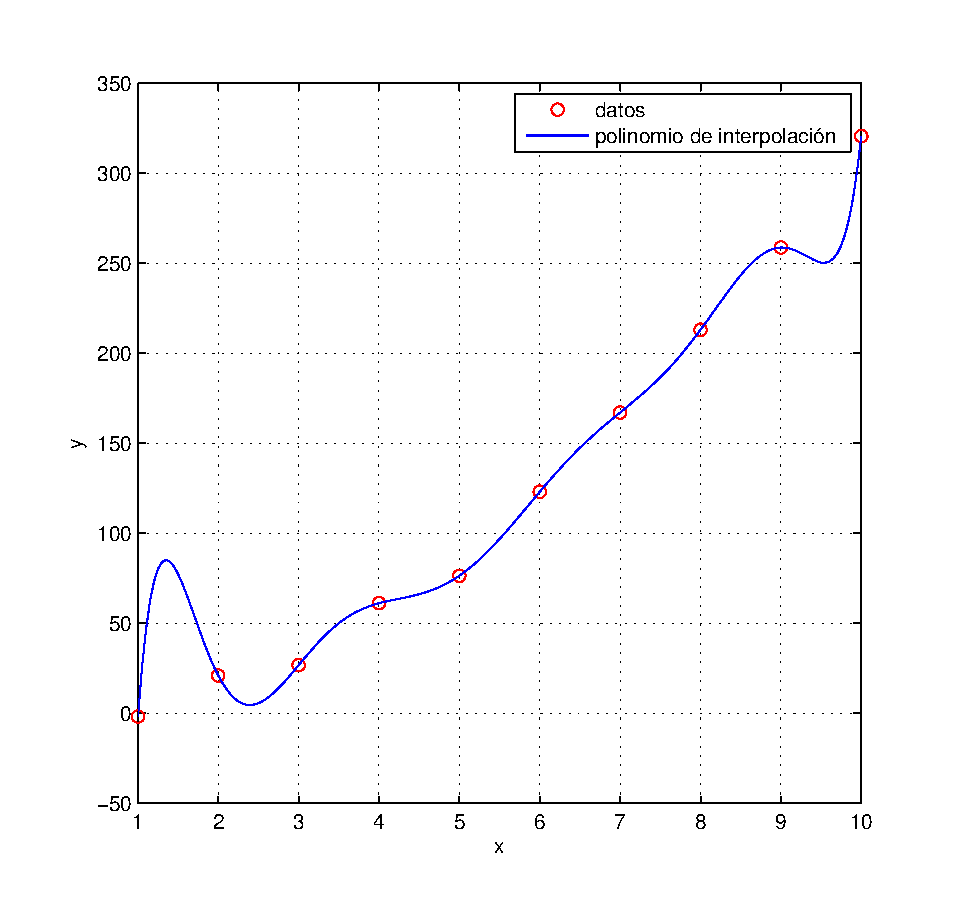
\includegraphics[width=10cm]{intpoli.eps}
\caption{Polinomio de interpolación de grado nueve obtenido a partir de un conjunto de diez datos} 
\label{fig:intepol}
\end{figure}
\begin{paracol}{2}
\section{Interpolación por intervalos.}
Hasta ahora, hemos visto cómo interpolar un conjunto de $n+1$ datos mediante un polinomio de grado $n$. En muchos casos, especialmente cuando el número de datos es suficientemente alto, los resultados de dicha interpolación pueden no ser satisfactorios.  La razón es que el grado del polinomio de interpolación crece linealmente con el número de puntos a interpolar, así por ejemplo para interpolar 11 datos necesitamos un polinomio de grado 10. Desde un punto de vista numérico, este tipo de polinomios pueden dar grandes errores debido al redondeo. Por otro lado, y dependiendo de la disposición de los datos para los que se realiza la interpolación, puede resultar que el polinomio obtenido tome una forma demasiado complicada para los valores comprendidos entres los datos interpolados..  

La figura \ref{fig:intepol} muestra el polinomio de interpolación de grado nueve para un conjunto de 10 datos. Es fácil darse cuenta, simplemente observando los datos, que no hay ninguna razón que justifique las curvas que traza el polinomio entre los puntos $1$ y $2$  o los puntos $9$ y $10$, por ejemplo.
\end{paracol}
\begin{figure}
\centering
\subfigure[Interpolación de orden cero  \label{fig:stepwise}]{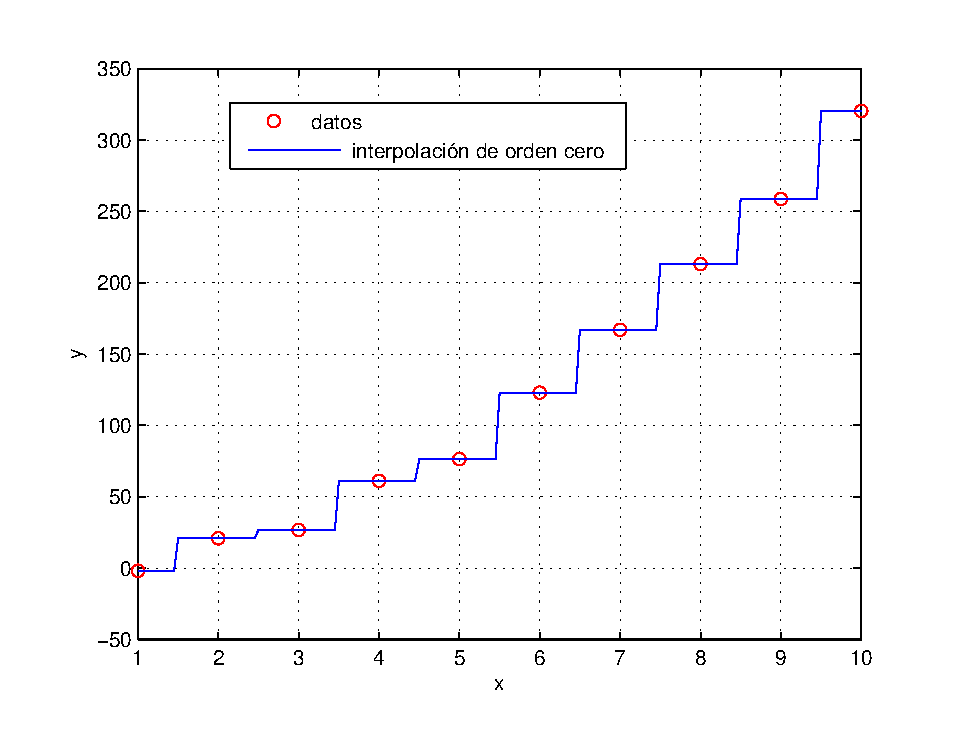
\includegraphics[width=7cm]{steps.eps}} %\qquad 
\subfigure[Interpolación lineal  \label{fig:lineal}]{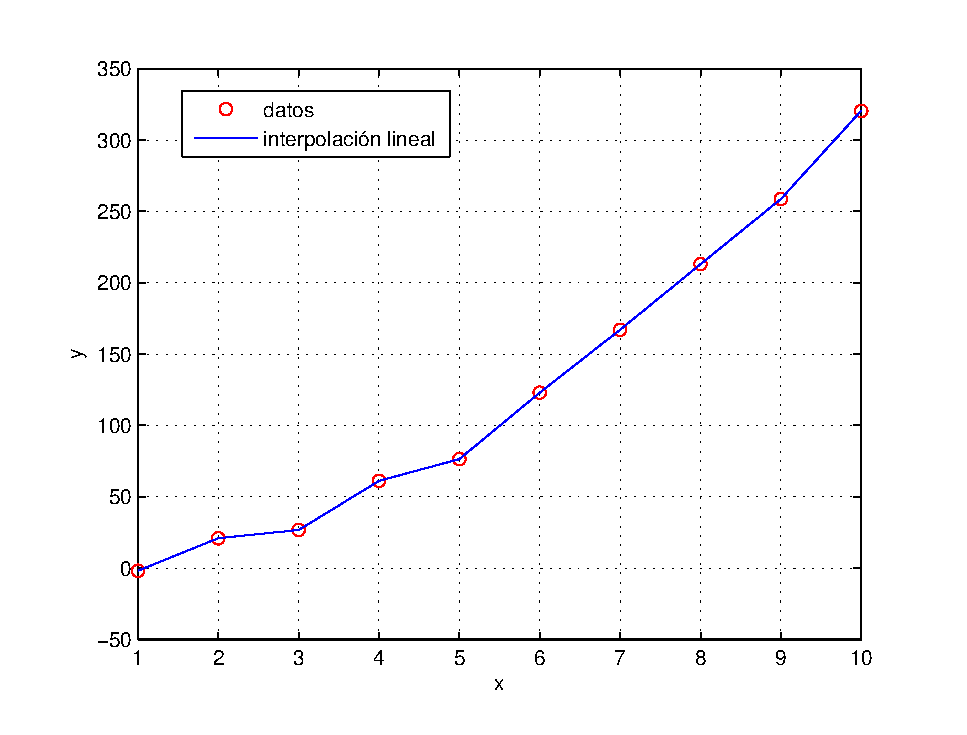
\includegraphics[width=7cm]{lineal.eps}}\\
\caption{Interpolaciones de orden cero y lineal para los datos de la figura \ref{fig:intepol} }
\end{figure}

\begin{paracol}{2}
En muchos casos es preferible no emplear todos los datos disponibles para obtener un único polinomio de interpolación. En su lugar, lo que se hace es dividir el conjunto de datos en varios grupos ---normalmente se agrupan formando intervalos de datos consecutivos--- y obtener varios polinomios de menor grado, de modo que cada uno interpole los datos de un grupo distinto. 

El grado de los polinomios empleados deberá estar, en principio, relacionado con los datos contenidos en cada tramo.


\paragraph{interpolación de orden cero} \index{Interpolación de orden cero} si hacemos que cada intervalo contenga un solo dato, obtendríamos polinomios de interpolación de grado cero, $a_{0i}=y_i$. El resultado, es un conjunto de escalones cuya valor varía de un intervalo a otro de acuerdo con el dato representativo contenido en cada tramo. La figura \ref{fig:stepwise} muestra el resultado de la interpolación de orden cero para los mismos diez datos de la figura \ref{fig:intepol}.

\paragraph{interpolación lineal.} \index{Interpolación lineal} En este caso, se dividen los datos en grupos de dos. Cada par de datos consecutivos se interpola calculando la recta que pasa por ellos. La interpolación lineal se emplea en muchas aplicaciones debido a su sencillez de cálculo. La figura \ref{fig:lineal}, muestra el resultado de aproximar linealmente los mismos datos contenidos en los ejemplos anteriores.

Siguiendo el mismo procedimiento, aumentando el número de datos contenidos en cada intervalo, podríamos definir una interpolación cuadrática, con polinomios de segundo grado, tomando intervalos que contengan tres puntos, una interpolación cúbica, para intervalos de cuatro puntos etc.

\subsection{Interpolación mediante splines cúbicos} \index{Interpolación!Splines}\index{Splines}
Hemos descrito antes cómo el polinomio interpolador de orden $n$ para un conjunto de $n+1$ datos puede presentar el inconveniente de complicar excesivamente la forma de  la curva obtenida entre los puntos interpolados. La interpolación a tramos que acabamos de describir, simplifica la forma de la curva entre los puntos pero presenta el problemas de la continuidad en las uniones entre tramos sucesivos. Sería deseable encontrar métodos de interpolación que fueran capaces de solucionar ambos problemas simultáneamente. Una buena aproximación a dicha solución la proporcionan los \emph{splines}.

Una función \emph{spline} está formado por un conjunto de polinomios, cada uno definido en un intervalo, que se unen entre sí obedeciendo a ciertas condiciones de continuidad.

Supongamos que tenemos una tabla de datos cualquiera,
\end{paracol}
\begin{table}[h]
\centering
\begin{tabular}{c|cccc}
x&$x_0$&$x_1$&$\cdots$&$x_n$\\
\hline
y&$y_0$&$y_1$&$\cdots$&$y_n$
\end{tabular}
\end{table}
\begin{paracol}{2}
Para construir una función \emph{spline} $S$ de orden $m$, que interpole los datos de la tabla, se definen intervalos tomando como extremos dos puntos consecutivos de la tabla y un polinomio de grado $m$ para cada uno de los intervalos,
\end{paracol}
\begin{equation*}
S= \left\{ 
\begin{aligned}
S_0(x),& \ x\in [x_0,x_1]\\
S_1(x),& \ x\in [x_1,x_2]\\
\vdots \\
S_i(x),& \ x\in [x_i,x_{i+1}]\\
\vdots \\
S_{n-1}(x),& \ x\in [x_{n-1},x_n]
\end{aligned}
\right.
\end{equation*}
\begin{paracol}{2}
Para que $S$ sea una función Spline de orden $m$ debe cumplir que sea continua y tenga $m-1$ derivadas continuas en el intervalo $[x_0,x_n]$ en que se desean interpolar los datos.
   
Para asegurar la continuidad, los polinomios que forman $S$ deben cumplir las siguientes condiciones en sus extremos;
\end{paracol}
\begin{align*}
S_i(x_{i+1})&=S_{i+1}(x_{i+1}),\ (1\leq i \leq n-1)\\
S'_i(x_{i+1})&=S'_{i+1}(x_{i+1}),\ (1\leq i \leq n-1)\\
S''_i(x_{i+1})&=S''_{i+1}(x_{i+1}),\ (1\leq i \leq n-1)\\
\vdots \\
S^{m-1}_i(x_{i+1})&=S^{m-1}_{i+1}(x_{i+1}),\ (1\leq i \leq n-1)\\
\end{align*}
\begin{paracol}{2}
Es decir, dos polinomios consecutivos del spline y sus $m-1$ primeras derivadas, deben tomar los mismos valores en el extremo común. 

Una consecuencia inmediata de las condiciones de continuidad exigidas a los splines es que sus derivadas sucesivas, $S',\ S'', \cdots$ son a su vez funciones spline de orden $m-1,\ m-2, \cdots$. Por otro lado, las condiciones de continuidad suministran  $(n-1)\cdot m$ ecuaciones que, unidas a las $n+1$ condiciones de interpolación ---cada polinomio debe pasar por los datos que constituyen los extremos de su intervalo de definición---,  suministran un total de  $n\cdot (m+1)-(m-1)$ ecuaciones. Este número es insuficiente para determinar los $(m+1)\cdot n$ parámetros correspondientes a los $n$ polinomios de grado $m$ empleados en la interpolación. Las $m-1$ ecuaciones que faltan se obtienen imponiendo a los splines condiciones adicionales.


\paragraph{Splines cúbicos.} \index{Splines! Cubicos} Los splines más empleados son los formados por polinomios de tercer grado. En total, tendremos que determinar $(m+1)\cdot n=4\cdot n$ coeficientes para obtener todos los polinomios que componen el spline. Las condiciones de continuidad más la de interpolación suministran en total $3\cdot (n-1)+n+1=4\cdot n-2$  ecuaciones. Necesitamos imponer al spline dos condiciones más. Algunas típicas son,
\begin{enumerate}
\item Splines naturales $S''(x_0)=S''(x_n)=0$
\item Splines con valor conocido en la primera derivada de los extremos $S'(x_0)=y'_0, S'(x_n)=y'_n$
\item Splines periódicos,
\begin{equation*}
\left\{ 
\begin{aligned}
S(x_0)&=S(x_n)\\
S'(x_0)&=S'(x_n)\\
S''(x_0)&=S''(x_n)
\end{aligned}
\right.
\end{equation*}
\end{enumerate}

Intentar construir un sistema de ecuaciones para obtener a la vez todos los coeficientes de todos los polinomios es una tarea excesivamente compleja porque hay demasiados parámetros.  Para abordar el problema partimos del hecho de que $S''(x)$ es también un spline de orden 1 para los puntos interpolados. Si los definimos como,
\end{paracol}
\begin{equation*}
S''_i(x)=-M_i\frac{x-x_{i+1}}{h_i}+M_{i+1}\frac{x-x_i}{h_i},\   i=0,\cdots, n-1
\end{equation*}

\begin{paracol}{2}
donde $h_i=x_{i+1}-x_i$ representa el ancho de cada intervalo y donde cada valor $M_i=S''(x_i)$ será una de las incógnitas que deberemos resolver.

Si integramos dos veces la expresión anterior,
\end{paracol}
\begin{align*}
S'_i(x)&=-M_i\frac{(x-x_{i+1})^2}{2\cdot h_i}+M_{i+1}\frac{(x-x_i)^2}{2\cdot h_i}+A_i,\   i=0,\cdots, n-1\\
S_i(x)&=-M_i\frac{(x-x_{i+1})^3}{6\cdot h_i}+M_{i+1}\frac{(x-x_i)^3}{6\cdot h_i}+A_i(x-x_i)+B_i,\   i=0,\cdots, n-1\\
\end{align*}
\begin{paracol}{2}
Empezamos por imponer las condiciones de interpolación: el polinomio $S_i$ debe pasar por el punto $(x_i,y_i)$,
\end{paracol}
\begin{equation*}
S_i(x_i)=-M_i\frac{(x_i-x_{i+1})^3}{6\cdot h_i}+B_i=y_i \Rightarrow B_i=y_i-\frac{M_i\cdot h_i^2}{6},\ i=0,\cdots, n-1
\end{equation*}
\begin{paracol}{2}
A continuación imponemos continuidad del spline en los nodos comunes: El polinomio $S_{i-1}$ también debe pasar por el punto $(x_i, y_i)$,
\end{paracol}
\begin{align*}
S_{i-1}(x_i)&=M_i\frac{(x_i-x_{i-1})^3}{6\cdot h_i}+A_{i-1}(x_i-x_{i-1})+\overbrace{y_{i-1}-\frac{M_{i-1}\cdot h_{i-1}^2}{6}}^{B_{i-1}}=y_i \Rightarrow\\
\Rightarrow A_{i-1}&=\frac{y_i-y_{i-1}}{h_{i-1}}-\frac{M_i-M_{i-1}}{6}\cdot h_{i-1}, \ i=1,\cdots, n
\end{align*}
\begin{paracol}{2}
Y por tanto,
\end{paracol}
\begin{equation*}
A_i=\frac{y_{i+1}-y_i}{h_i}-\frac{M_{i+1}-M_i}{6}\cdot h_i, \ i=0,\cdots, n-1
\end{equation*}
\begin{paracol}{2}
En tercer lugar imponemos la condición de que las derivadas también sean continuas en los nodos comunes,
\end{paracol}
\begin{align*}
S'_i(x_i)&=-M_i\frac{(x_i-x_{i+1})^2}{2\cdot h_i}+M_{i+1}\frac{(x_i-x_i)^2}{2\cdot h_i}+\frac{y_{i+1}-y_i}{h_i}-\frac{M_{i+1}-M_i}{6}\cdot h_i,\   i=0,\cdots, n-1\\
S'_{i-1}(x_i)&=-M_{i-1}\frac{(x_i-x_i)^2}{2\cdot h_{i-1}}+M_{i}\frac{(x_i-x_{i-1})^2}{2\cdot h_{i-1 }}+\frac{y_i-y_{i-1}}{h_{i-1}}-\frac{M_i-M_{i-1}}{6}\cdot h_{i-1},\   i=1,\cdots, n\\
S'_i(x_i)&=S'_{i-1}(x_i) ,\   i=1,\cdots, n-1 \Rightarrow\\
&\Rightarrow -M_i\frac{h_i}{2}+\frac{y_{i+1}-y_i}{h_i}-\frac{M_{i+1}-M_i}{6}\cdot h_i=M_{i}\frac{h_{i-1}}{2}+\frac{y_i-y_{i-1}}{h_{i-1}}-\frac{M_i-M_{i-1}}{6}\cdot h_{i-1}
\end{align*}
\begin{paracol}{2}
Si agrupamos a un lado los valores $M_{i-1}, M_i, M_{i+1}$,
\end{paracol}
\begin{align*}
h_{i-1}\cdot M_{i-1}+2\cdot (h_{i-1}+h_i)\cdot M_i+h_i\cdot M_{i+1}=6\cdot \left(\frac{y_{i+1}-y_i}{h_i}-\frac{y_i-y_{i-1}}{h_{i-1}}\right)\\
i=1,\cdots ,n-1
\end{align*}
\begin{paracol}{2}
En total tenemos $M_0,\cdots, M_n$, $n+1$ incógnitas y la expresión anterior, solo nos suministra $n-1$ ecuaciones. Necesitamos dos ecuaciones más, Si imponemos la condición de splines naturales, Para el extremo de la izquierda del primer polinomio y para el extremo de la derecha del último,
\end{paracol}
\begin{align*}
M_0=S''(x_0)=0\\
M_n=S''(x_n)=0
\end{align*}
\begin{paracol}{2}
Con estas condiciones y la expresión obtenida para el resto de los $M_i$, podemos construir un sistema de ecuaciones tridiagonal
\end{paracol}
\begin{equation*}
\begin{pmatrix}
2(h_0+h_1) & h_1 & 0 &0&\cdots &0&0\\
 h_1 & 2(h_1+h_2) & h_2 &0& \cdots&0 & 0\\
0& h_2 & 2(h_2+h_3) & h_3 &\cdots &0& 0\\
\vdots & \vdots & \vdots &\vdots& \ddots & \vdots&\vdots \\
0 & 0 & 0&0&\cdots& 2(h_{n-3}+h_{n-2}) & h_{n-2} \\ 
0 & 0 & 0&0&\cdots&h_{n-2} & 2(h_{n-2}+h_{n-1})
\end{pmatrix}\cdot \begin{pmatrix}
M_1\\
M_2\\
M_3\\
\vdots \\
M_{n-1}
\end{pmatrix}=\begin{pmatrix}
b_1\\
b_2\\
b_3\\
\vdots \\
b_{n-1}
\end{pmatrix}
\end{equation*}
\begin{paracol}{2}
Donde hemos hecho,
\end{paracol}
\begin{equation*}
b_i=6\cdot \left(\frac{y_{i+1}-y_i}{h_i}-\frac{y_i-y_{i-1}}{h_{i-1}}\right)
\end{equation*}
\begin{paracol}{2}
Tenemos un sistema de ecuaciones en el que la matriz de coeficientes es tridiagonal y además diagonal dominante, por lo que podríamos emplear cualquiera de los métodos vistos en capítulo  
\ref{sistemas}.  Una vez resuelto el sistema y obtenidos los valores de $M_i$, obtenemos los valores de $A_i$ y $B_i$ a Partir de las ecuaciones obtenidas más arriba.

Por último, la forma habitual de definir el polinomio de grado 3 $S_i$, empleado para interpolar los valores del intervalo $[x_i,x_{i+1}]$, mediante splines cúbicos se define como, 
\end{paracol}
\begin{equation*}
S_i(x)=\alpha_i+\beta_i(x-x_i)+\gamma_i(x-x_i)^2+\delta_i(x-x_i)^3, \ x\in [x_i,x_{i+1}],\ (i=0,1,\cdots,n-1)
\end{equation*}
\begin{paracol}{2}
Donde,
\end{paracol}
\begin{align*}
\alpha_i &=y_i\\
\beta_i &=\frac{y_{i+1}-y_i}{h_i}-\frac{M_i \cdot h_i}{3}-\frac{M_{i+1} \cdot h_i}{6}\\
\gamma_i &=\frac{M_i}{2}\\
\delta_i &=\frac{M_{i+1}-M_i}{6\cdot h_i}
\end{align*}
\begin{paracol}{2}
La siguiente función permite obtener los coeficientes y el resultado de interpolar un conjunto de puntos mediante splines cúbicos,
\end{paracol}
%\begin{lstlisting}
%function [c,yi]=spcubic(x,y,xi)
% uso [c,yi]=spcubic(x,y,xi)
% Esta funci?n interpola los puntos contenidos en los vectores columna x e y
% empleando parae ello splines c?bicos naturales. devuelve los coeficientes
% de los polinomios en una matriz de dimension (n-1)*4. Cada fila contiene
% un splin desde So a Sn-1 los coeficiente est?n guardados el la fila en
% orden depotencia creciente: ejemplo c(i,1)+c(i,2)*x+c(i,3)*x^2+c(i,4)*x^3
% ademas devuelve los valores interpolados yi correspondientes a puntos xi
% contenidos en el intervalo definido por los valores de x

% obtenemos la longitud de los datos...
%l=length(x);
% obtencion de los coeficientes M
% Construimos el vector de diferencias h y un vector de diferencias
% Dy=y(i+1)-y(i) Que nos ser? muy ?til a la hora de calcular el vector de
% t?rminos independientes del sistema

%for i=1:l-1
%    h(i)=x(i+1)-x(i);
%    Dy(i)=y(i+1)-y(i);
%end

% Construimos la matriz del sistema. (Lo ideal seria definirla como una
% matriz sparse pero en fin no sabeis, porque sois todav?a peque?os, etc...)

%CSP(l-2,l-2)=2*(h(l-2)+h(l-1));
%b(l-2,1)=6*(Dy(l-1)/h(l-1)-Dy(l-2)/h(l-2));
%for i=1:l-3
%    CSP(i,i)=2*(h(i)+h(i+1));
%    CSP(i,i+1)=h(i+1);
%    CSP(i+1,i)=h(i+1);
%    b(i,1)=6*(Dy(i+1)/h(i+1)-Dy(i)/h(i));
%end

% calculamos los coeficientes M,
%M=CSP\b;

% A?adimos el primer y el ?ltimo valor como ceros (Splines naturales)
%M=[0;M;0];

% calulamos los coeficientes A,
%for i=1:l-1
%    A(i)=Dy(i)/h(i)-(M(i+1)-M(i))*h(i)/6;
%end
% Calculamos los coeficientes B,
%for i=1:l-1
%    B(i)=y(i)-M(i)*h(i)^2/6;
%end
% Podemos ahora calcular el valor que toma el polinomio para los puntos
% que se desea interpolar

% miramos cuantos puntos tenemos
%l2=length(xi);
%for i=1:l2
    % miramos en que intervalo esta el punto xi(i)
%    j=1;
%    while xi(i)>x(j)
%        j=j+1;
%    end
%    if j>l-1
%        j=l-1; % aunque estamos extrapolando
%    elseif j<2
%        j=2; % estamos calculando el primer punto o estamos tanbien
        % extrapolando
%    end
    
%    yi(i)=-M(j-1)*(xi(i)-x(j))^3/(6*h(j-1))+...
%        M(j)*(xi(i)-x(j-1))^3/(6*h(j-1))+A(j-1)*(xi(i)-x(j-1))+B(j-1);
%end

% calcumos los coeficientes c del spline en forma 'normal'
% la primera columna, son los valores de i,
%c=zeros(l-1,4);
%for i=1:l-1
%    c(i,1)=y(i);
%    c(i,2)=Dy(i)/h(i)-M(i)*h(i)/3-M(i+1)*h(i)/6;
%    c(i,3)=M(i)/2;
%    c(i,4)=(M(i+1)-M(i))/(6*h(i));
%end
%\end{lstlisting}


\begin{paracol}{2}
 La figura, \ref{fig:splines} muestra el resultado de interpolar mediante un spline cúbico, los datos contenidos en la figura \ref{fig:intepol}. Es fácil observar cómo ahora los polinomios de interpolación dan como resultado una curva suave en los datos interpolados y en la que además las curvas son también suaves, sin presentar variaciones extrañas, para los puntos contenidos en cada intervalo entre dos datos.
\end{paracol}

\begin{figure}[h]
\centering
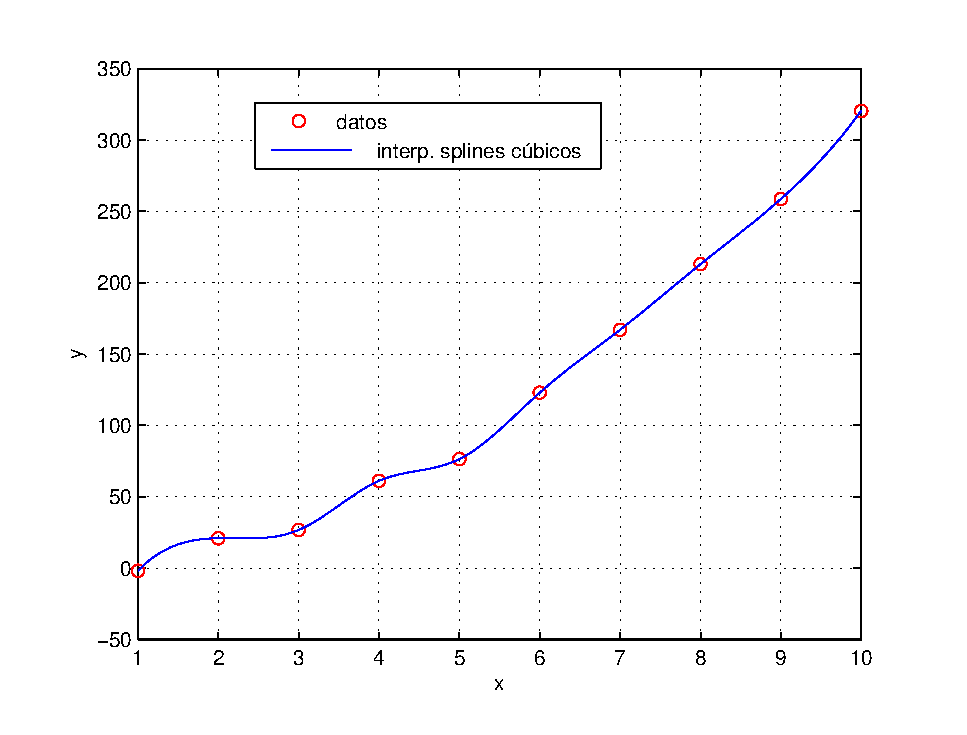
\includegraphics[width=12cm]{splines.eps}
\caption{Interpolación mediante spline cúbico de los datos de la figura \ref{fig:intepol}} 
\label{fig:splines}
\end{figure} 
 
\begin{paracol}{2} 
\subsection{Funciones propias de Matlab para interpolación por intervalos} \index{interp1@\texttt{interp1}}

Para realizar una interpolación por intervalos mediante cualquiera de los procedimientos descritos, Matlab incorpora la función propia \texttt{interp1}. Esta función admite como variables de entrada dos vectores con los valores de las coordenadas $x$ e $y$ de los datos que se desea interpolar y un tercer vector $x1$ con los puntos para los que se desea calcular el valor de la interpolación. Además, admite como variable  de entrada una cadena de caracteres que indica el método con el que se quiere realizar la interpolación. Dicha variable puede tomar los valores:
\begin{enumerate}
\item \texttt{'nearest'}. Interpola el intervalo empleando el valor $y_i$ correspondiente al valor  $x_i$ más cercano al punto que se quiere interpolar. El resultado es una interpolación a escalones.
\item \texttt{'linear'} realiza una interpolación lineal entre los puntos del conjunto de datos que se desea interpolar.
\item \texttt{'spline'}. Interpola empleando splines cúbicos naturales.
\item \texttt{'cubic'} o \texttt{'pchip} Emplea polinomios de Hermite cúbicos. Es un método similar al de los splines que no describiremos en estos apuntes.
\end{enumerate} 

La función devuelve como salida los valores interpolados correspondientes a los puntos de $x1$. El siguiente código muestra el modo de usar el comando \texttt{interp1}. Para probarlo se han creado dos vectores \texttt{x} e \texttt{y} que contienen el conjunto de datos que se empleará para calcular la interpolación. Además, se ha creado otro vector \texttt{x1} que contiene los puntos para los que se quiere calcular el resultado de la interpolación.
\end{paracol}
\begin{verbatim}
>> x=[1:2:16]
x =
     1     3     5     7     9    11    13    15
>> y=[1 3 4 2 -1 4 -5 3]
y =
     1     3     4     2    -1     4    -5     3
>> x1=[3.5 7.5]
x1 =
    3.5000    7.5000
>> y1=interp1(x,y,x1,'spline')
y1 =
    3.4110    0.7575
>> x=[1:2:16]
x =
     1     3     5     7     9    11    13    15
>> y=[1 3 4 2 -1 4 -5 3]
y =
     1     3     4     2    -1     4    -5     3
>> x1=[3.5 7.5]
x1 =
    3.5000    7.5000
>> y1=interp1(x,y,x1,'nearest')
y1 =
     3     2
>> y1=interp1(x,y,x1,'linear')
y1 =
    3.2500    1.2500
>> y1=interp1(x,y,x1,'cubic')
y1 =
    3.3438    1.1938
\end{verbatim}
\begin{paracol}{2}
\section{Ajuste polinómico por el método de mínimos cuadrados}\label{sec:mc}\index{Mínimos cuadrados} \index{Ajuste polinómico}
Los métodos de interpolación que hemos descrito en las secciones anteriores pretenden encontrar un polinomio o una función definida a partir de polinomios que pase por un conjunto de datos. En el caso del ajuste por mínimos cuadrados, lo que se pretende es buscar el polinomio, de un grado dado, que mejor se aproxime a un conjunto de datos.

Supongamos que tenemos un conjunto de $m$ datos, 
\end{paracol}
\begin{table}[h]
\centering
\begin{tabular}{c|cccc}
x&$x_1$&$x_2$&$\cdots$&$x_m$\\
\hline
y&$y_1$&$y_2$&$\cdots$&$y_m$
\end{tabular}
\end{table} 
\begin{paracol}{2}
Queremos construir un polinomio $p(x)$  de grado $n < m-1$, de modo que los valores que toma el polinomio para los datos $p(x_i)$ sean lo más cercanos posibles a los correspondientes valores $y_i$. 

En primer lugar, necesitamos clarificar qué entendemos por \emph{lo más cercano posible}.  Una posibilidad, es medir la diferencia, $y_i-p(x_i)$ para cada par de datos del conjunto. Sin embargo, es más frecuente emplear el cuadrado de dicha diferencia, $\left(y_i-p(x_i)\right)^2$. Esta cantidad tiene, entre otras, la ventaja de que su valor es siempre positivo con  independencia de que la diferencia sea positiva o negativa. Además, representa el cuadrado de la distancia entre $p(x_i)$ e $y_i$. Podemos tomar la suma de dichas distancias al cuadrado, obtenidas por el polinomio para todos los pares de puntos, 
\end{paracol}
\begin{equation*}
\sum_{i=1}^m \left(y_i-p(x_i)\right)^2
\end{equation*}
\begin{paracol}{2}
\noindent como una medida de la distancia del polinomio a los datos.  De este modo,  el polinomio \emph{lo más cercano posible}  a los datos sería aquel que minimice la suma de diferencias al cuadrado que acabamos de definir. De ahí el nombre del método.

En muchos casos, los datos a los que se pretende ajustar un polinomio por mínimos cuadrados son datos experimentales. En función del entorno experimental y del método con que se han adquirido los datos, puede resultar que algunos resulten más fiables que otros. En este caso, sería deseable hacer que el polinomio se aproxime más a los datos más fiables. Una forma de hacerlo es añadir unos \emph{pesos}, $\omega_i$, a las diferencias al  cuadrado en función de la confianza que nos merece cada dato,
\end{paracol}
\begin{equation*}
\sum_{i=1}^m \omega_i \left(y_i-p(x_i)\right)^2
\end{equation*}
\begin{paracol}{2}
Los datos fiables se multiplican por valores de $\omega$ grandes y los poco fiables por valores pequeños.

Para ver cómo obtener los coeficientes de un polinomio de mínimos cuadrados, empezaremos con el caso más sencillo; un polinomio de grado $0$. En este caso, el polinomio es una constante, definida por su término independiente $p(x)=a_0$. El objetivo a minimizar sería entonces,
\end{paracol}
\begin{equation*}
g(a_0)=\sum_{i=1}^m \omega_i \left(y_i-a_0\right)^2
\end{equation*}
\begin{paracol}{2}
El valor mínimo de esta función debe cumplir que su derivada primera $g'(a_0)=0$ y que su derivada segunda  $g''(a_0)\geq 0$,
\end{paracol}
\begin{align*}
g'(a_0)&=-2\sum_{i=1}^m \omega_i \left(y_i-a_0\right)=0 \Rightarrow a_0=\frac{\sum_{i=1}^m \omega_i\cdot y_i}{ \sum_{i=1}^m \omega_i}\\
g''(a_0)&=2\sum_{i=1}^m \omega_i \Rightarrow  g''(a_0) \geq 0
\end{align*}
\begin{paracol}{2}
El resultado obtenido para el valor de $a_0$ es una media, ponderada con los pesos $w_i$ de los datos. Si hacemos $w_i=1 \ \forall w_i$ obtendríamos exactamente la media de los datos. Este resultado resulta bastante razonable. Aproximar un conjunto de valores por un polinomio de grado cero, es tanto como suponer que la variable $y$ permanece constante para cualquier valor de $x$. Las diferencias observadas deberían deberse entonces a errores aleatorios experimentales, y la mejor estima del valor de $y$ será precisamente el valor medio de los valores disponibles. La figura \ref{fig:mc0} muestra el resultado de  calcular el polinomio de mínimos cuadrados de grado cero para un conjunto de datos.
\end{paracol}
\begin{figure}[h]
\centering
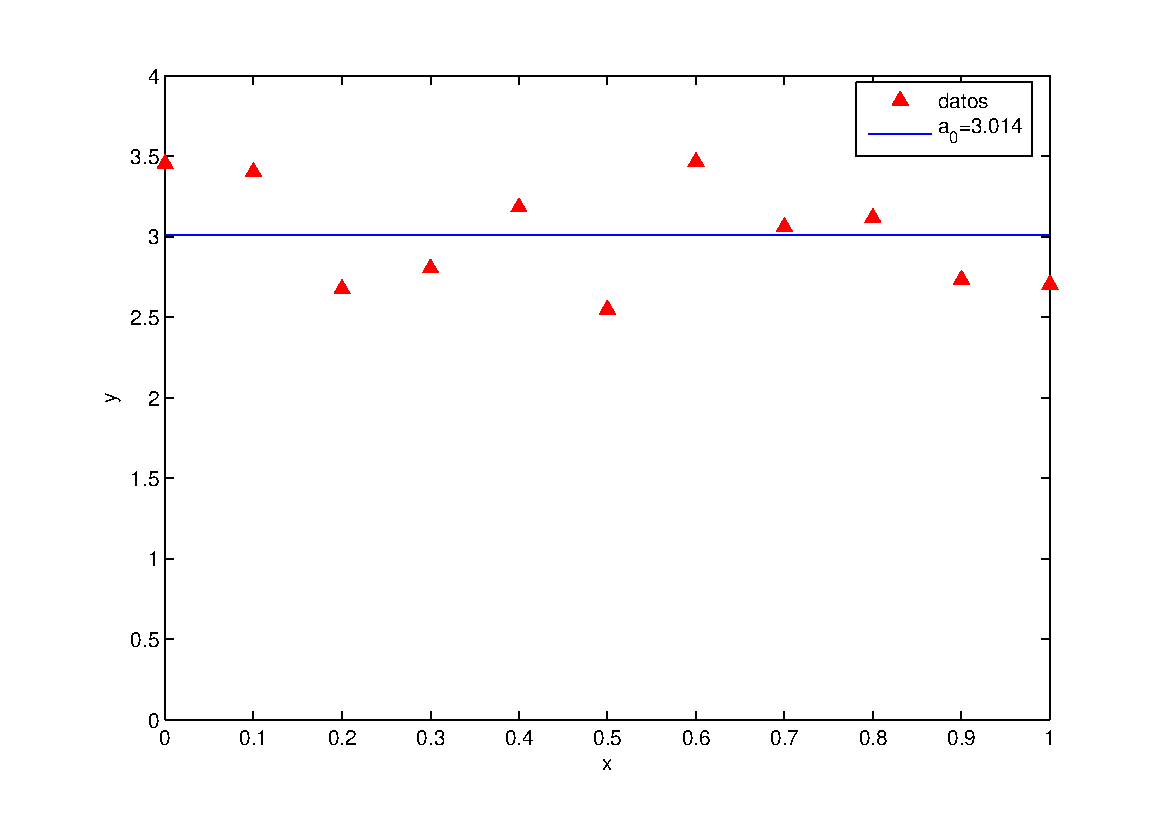
\includegraphics[width=12cm]{mc0.eps}
\caption{Polinomio de mínimos cuadrados de grado 0} 
\label{fig:mc0}
\end{figure} 
\begin{paracol}{2}
El siguiente paso en dificultad sería tratar de aproximar un conjunto de datos por un polinomio de grado 1, es decir, por una linea recta, $p(x)=a_0+a_1 x$. En este caso, la suma de diferencias al cuadrado toma la forma,
\end{paracol}
\begin{equation*}
g(a_0,a_1)=\sum_{i=1}^m \omega_i\left(y_i-a_0-a_1 x_i \right)^2
\end{equation*}
\begin{paracol}{2} 
En este caso, tenemos dos coeficientes sobre los que calcular el mínimo. Éste se obtiene cuando las derivadas parciales de $g(a_0,a_1)$ respecto a ambos coeficientes son iguales a cero. 
\end{paracol}
\begin{align*}
\frac{\partial g}{\partial a_0}&=-2\sum_{i=1}^m \omega_i (y_i-a_0-a_1 x_i) = 0\\
\frac{\partial g}{\partial a_1}&=-2\sum_{i=1}^m \omega_i x_i(y_i-a_0-a_1 x_i) = 0
\end{align*} 
\begin{paracol}{2}
Si reordenamos las ecuaciones anteriores, 
\end{paracol}
\begin{align*}
&\left(\sum_{i=1}^m \omega_i\right)a_0+ \left(\sum_{i=1}^m \omega_ix_i\right)a_1 =\sum_{i=1}^m \omega_iy_i\\
&\left(\sum_{i=1}^m \omega_ix_i\right)a_0+ \left(\sum_{i=1}^m \omega_ix_i^2\right)a_1 =\sum_{i=1}^m \omega_ix_iy_i
\end{align*}
\begin{paracol}{2}
Obtenemos un sistema de dos ecuaciones lineales cuyas incógnitas son precisamente los coeficientes de la recta de mínimos cuadrados.

Podemos ahora generalizar el resultado para un polinomio de grado $n$, $p(x)=a_0+a_1x+a_2x^2+\cdots +a_nx^n$. La función $g$ toma la forma,
\end{paracol}
\begin{equation*}
g(a_0,a_1,\cdots, a_n)=\sum_{i=1}^m \omega_i \left (a_0+a_1x_i+\cdots+ a_nx_i^n-y_i\right)^2
\end{equation*}
\begin{paracol}{2}
De nuevo, para obtener los coeficientes del polinomio igualamos las derivadas parciales a cero,
\end{paracol}
\begin{equation*}
\frac{\partial g(a_0,a_1,\cdots, a_n)}{\partial a_j}=0 \Rightarrow \sum_{i=1}^m \omega_i x_i^j \left( a_0+a_1x_i+\cdots + a_nx_i^n-y_i\right)=0, \ j=0,1\cdots, n
\end{equation*} 
\begin{paracol}{2}
Si reordenamos las expresiones anteriores, llegamos a un sistema de $n+1$ ecuaciones lineales, cuyas incógnitas son los coeficientes del polinomio de mínimos cuadrados,
\end{paracol}
\begin{equation*}
\begin{pmatrix}
s_0& s_1& \cdots s_n\\
s_1& s_2& \cdots s_{n+1}\\
\vdots & \vdots & \ddots \\
s_n& s_{n+1}& \cdots s_{2n}\\
\end{pmatrix}\cdot \begin{pmatrix}
a_0\\
a_1\\
\vdots \\
a_n
\end{pmatrix}=\begin{pmatrix}
c_0\\
c_1\\
\vdots \\
c_n
\end{pmatrix}
\end{equation*} 
\begin{paracol}{2}
Donde hemos definido $s_j$ y $c_j$ como,
\end{paracol}
\begin{align*}
s_j&=\sum_{i=1}^m \omega_ix_i^j\\
c_j&=\sum_{i=1}^m \omega_ix_i^jy_i
\end{align*}
\begin{paracol}{2} 
El siguiente código permite obtener el polinomio de mínimos cuadrados que aproxima un conjunto de $n$ datos,
\end{paracol}
%\begin{lstlisting}
%function a=mc(x,y,n,w)
%% uso: a=mc(x,y,n,w). Esta función permite obtener los coeficientes del
%% polinomio de mínimos cuadrados que ajusta un conjunto de datos. Las
%% variables de entrada son: x, vector con la componente x de los datos a
%% ajustar. y, vector con la componente y de los datos a ajustar. n grado del
%% polinomio de minimos cuadrados. w vector de pesos asociados a los datos. si no
%% se sumininstra se toman todos los pesos como 1. Salidas: vector columna con
%% los coeficientes del polinomio=> a(1)+a(2)*x+a(3)*x^2+a(n+1)*x^n
%
%% comprobamos en primer lugar que tenemos datos suficientes,
%
%m=length(x);
%if m<n+1
%    error('no hay datos sufiecientes para calcular el polinomio pedido')
%end
%% Si no se ha suministrado vector de pesos construimos uno formado por unos,
%if nargin < 4
%	w=ones(m,1);
%end
%% Montamos un bucle para crear los elementos s de la matriz de coeficientes,
%for j=1:2*n+1
%    s(j)=0;    
%for i=1:m
%    s(j)=s(j)+w(i)*x(i)^(j-1);
%end
%end
%
%
%% y un segundo bucle para crear los términos independientes...
%for j=1:n+1
%    c(j,1)=0;
%    for i=1:m
%        c(j,1)=c(j,1)+w(i)*x(i)^(j-1)*y(i)
%    end
%end
%
%%  a partir de los valores de s, construimos la matriz del sistema,
%for i=1:n+1
%    for j=1:n+1
%        A(i,j)=s(i+j-1)
%    end
%end
%
%% solo nos queda resolver el sistema... Empleamos la division por la
%% izquierda de matlab
%
%a=A\c;
%\end{lstlisting}
\begin{paracol}{2}
Una última observación importante es que si intentamos calcular el polinomio de mínimos cuadrados de grado $m-1$ que aproxima un conjunto de $m$ datos, lo que obtendremos será el polinomio de interpolación. En general, cuanto mayor sea el grado del polinomio más posibilidades hay de que la matriz de sistema empleado para obtener los coeficientes del polinomio esté mal condicionada.

\subsection{Mínimos cuadrados en Matlab.}

Matlab suministra dos maneras distintas de ajustar un polinomio a unos datos por mínimos cuadrados. La primera es mediante el uso del comando \texttt{polyfit}. Este comando admite como entradas un vector de coordenadas $x$ y otro de coordenadas $y$, de los datos que se quieren aproximar, y una tercera variable con el grado del polinomio. Como resultado devuelve un vector con los coeficientes del polinomio de mínimos cuadrados. Ordenados en orden de potencias decrecientes \texttt{a(1)*x\^\  n+a(2)*x\^\  (n-1)+...+a(n+1)}. La siguiente secuencia de comandos crea un par de vectores y muestra como manejar el comando,
\end{paracol}


\begin{verbatim}>> x=[1:10]
x =
     1     2     3     4     5     6     7     8     9    10
>> y=[-1 0 3 4 5.2 6 10 12 13 15.5];
>> a=polyfit(x,y,3)
a =
    0.0001    0.0411    1.3774   -2.4133
\end{verbatim}
\begin{paracol}{2}
A continuación, podemos emplear el comando \texttt{polyval}, para obtener en valor del polinomio de mínimos cuadrados obtenido en cualquier punto. En particular, si lo aplicamos a los datos $x$,
\end{paracol}
\begin{verbatim}
>> yhat=polyval(a,x)
yhat =
  Columns 1 through 7
   -0.9947    0.5067    2.0913    3.7596    5.5121    7.3491    9.2713
  Columns 8 through 10
   11.2790   13.3727   15.5529
\end{verbatim}
\begin{paracol}{2}
Por último, podemos calcular el error cometido por el polinomio $e_i=\vert p(x_i-y_i \vert$
\end{paracol}
\begin{verbatim}
>> error=abs(yhat-y)
error =
  Columns 1 through 7
    0.0053    0.5067    0.9087    0.2404    0.3121    1.3491    0.7287
  Columns 8 through 10
    0.7210    0.3727    0.0529
\end{verbatim}
\begin{paracol}{2}
Además del comando \texttt{polyfit} Matlab permite ajustar un polinomio por mínimos cuadrados a un conjunto de datos a través de la ventana gráfica de Matlab. Para ello, es suficiente representar los datos con el comando \texttt{plot(x,y)}. Una vez que Matlab muestra la ventana gráfica con los datos representados, se selecciona en el menú desplegable \texttt{tools} la opción \texttt{Basic Fitting}. Matlab abre una segunda ventana que permite seleccionar el polinomio de mínimos cuadrados que se desea ajustar a los datos, así como otras opciones que permiten obtener los coeficientes del polinomio y analizar la bondad del ajuste a partir de los residuos (ver sección siguiente). La figuras \ref{fig:minimos}, muestra un ejemplo de uso de la ventana gráfica de Matlab para obtener un ajuste por mínimos cuadrados 

\subsection{Análisis de la bondad de un ajuste por mínimos cuadrados.} \index{Mínimos cuadrados! Residuos}
Supongamos que tenemos un conjunto de datos obtenidos como resultado de un experimento. En muchos casos la finalidad de un ajuste por mínimos cuadrados, es encontrar una ley que nos permita relacionar los datos de la variable independiente con la variable dependiente. Por ejemplo si aplicamos distintas fuerzas a muelle y medimos la elongación sufrida por el muelle, esperamos obtener, en primera aproximación una relación lineal: $\Delta x\propto F$. (Ley de Hooke). 

Sin embargo, los resultados de un experimento no se ajustan nunca exactamente a una ley debido a errores aleatorios que no es posible corregir.

Cuando realizamos un ajuste por mínimos cuadrados, podemos emplear cualquier polinomio desde grado $0$ hasta grado $m-1$. Desde el punto de vista del error cometido con respecto a los datos disponibles el mejor polinomio sería precisamente el de grado $m-1$ que da error cero para todos los datos, por tratarse del polinomio de interpolación. Sin embargo, si los datos son experimentales estamos incluyendo los errores experimentales en el ajuste.

Por ello, para datos experimentales y suponiendo que los datos solo contienen errores aleatorios, el mejor ajuste lo dará el polinomio de menor grado para el cual las diferencias entre los datos y el polinomio $y_i-p(x_i)$ se distribuyan aleatoriamente. Estas diferencias reciben habitualmente el nombre de residuos. \index{Residuos} 
\end{paracol}
\begin{figure}[h]
\centering
\subfigure[Menu desplegable para abrir ventana auxiliar  \label{fig:minimos1}]{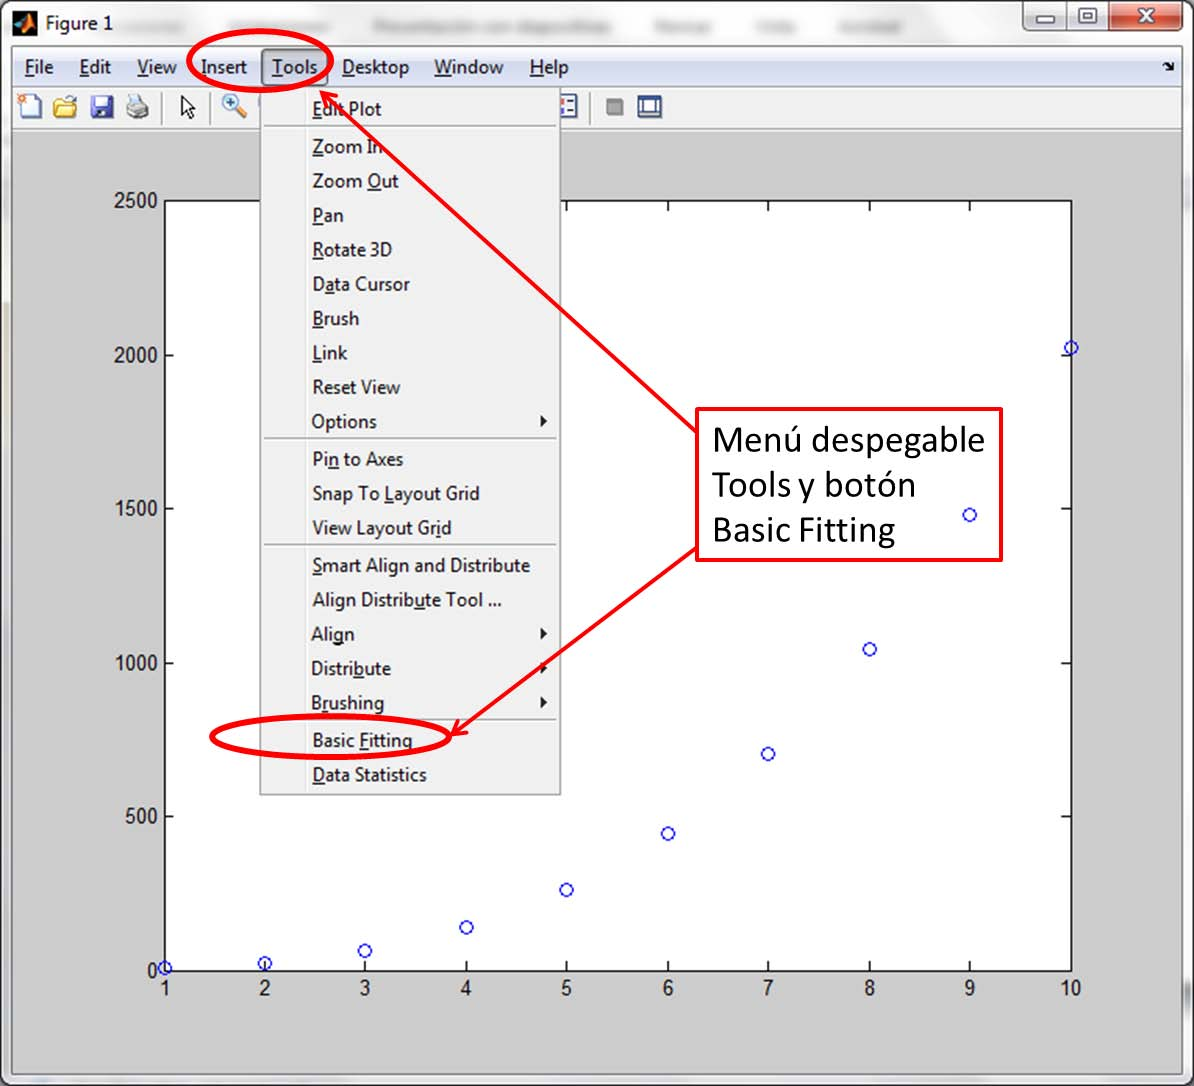
\includegraphics[width=5cm]{minimos.pdf}} \qquad 
\subfigure[ventana auxiliar para realizar el ajuste y analizar resultados  \label{fig:minimos2}]{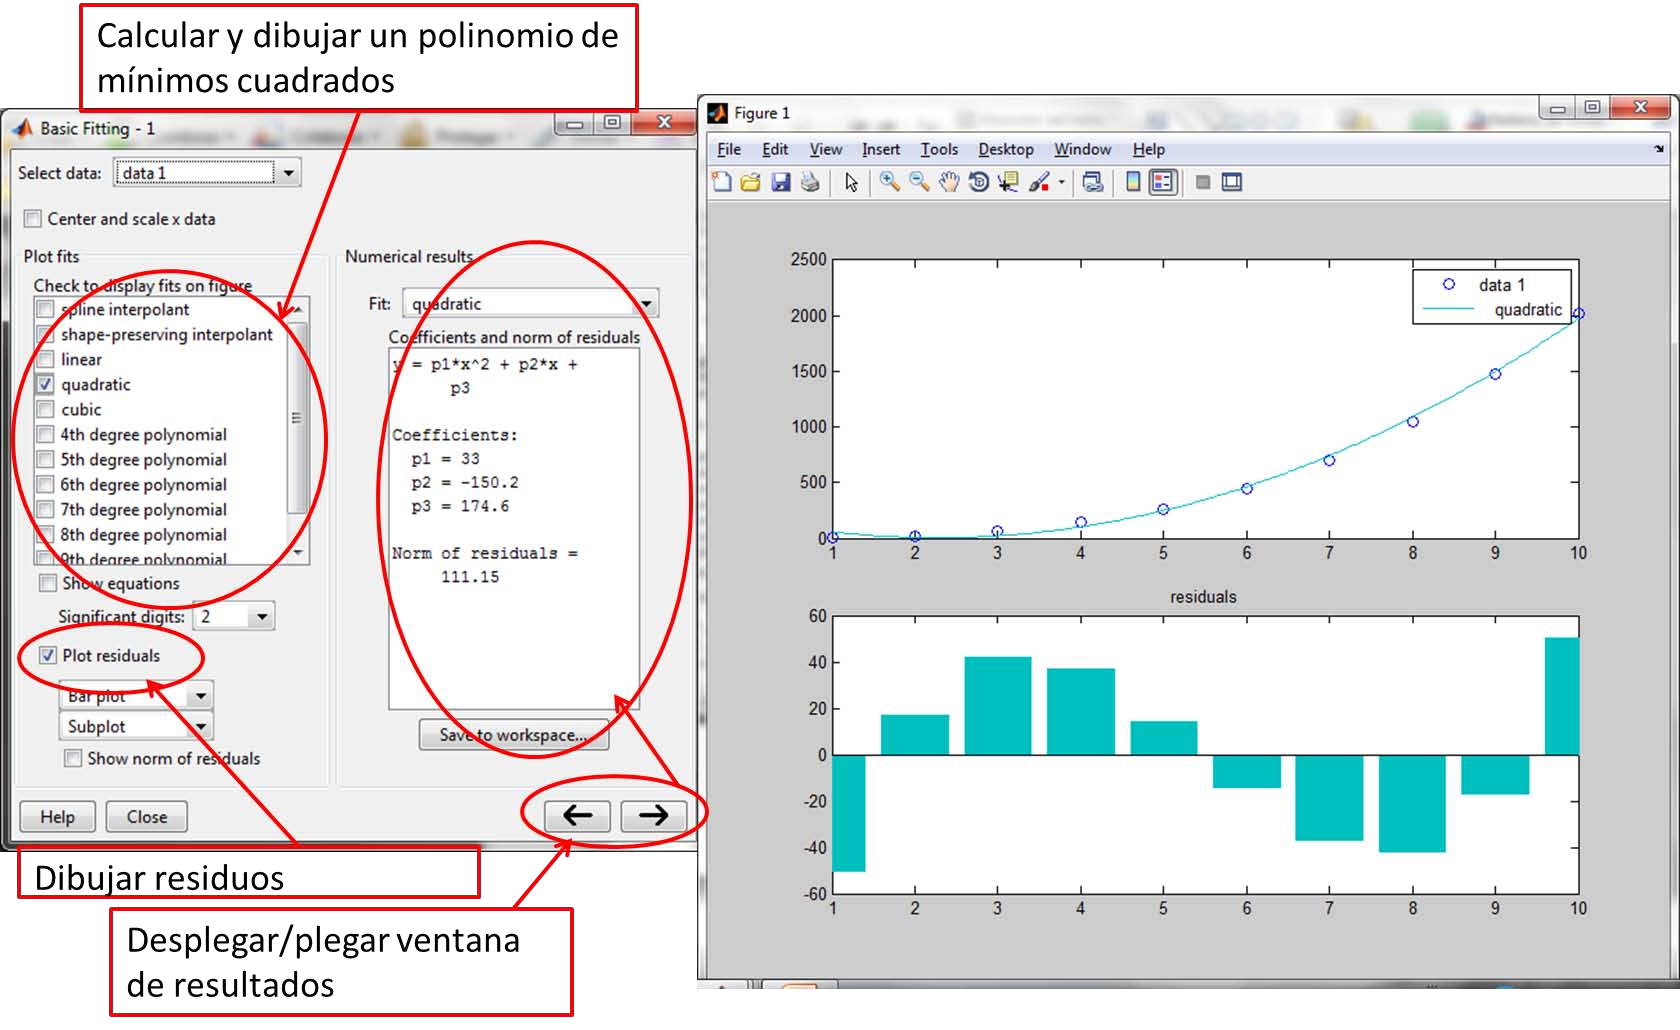
\includegraphics[width=10cm]{minimos2.pdf}}\\
\caption{Ejemplo de uso de la ventana gráfica de Matlab para realizar un ajuste por mínimos cuadrados}
\label{fig:minimos}
\end{figure}

\begin{paracol}{2}
Entre las herramientas que suministra la ventanas gráficas de Matlab para el ajuste por mínimos cuadrados hay una que calcula y representa los residuos.  La figura \ref{fig:residuos} muestra un ejemplo de ajuste por mínimos cuadrados empleando cada vez un polinomio de mayor grado. \index{Residuos!Cálculo con Matlab}
  
  
En la figura \ref{fig:residuos1} se observa claramente que el ajusto no es bueno, la recta de mínimos cuadrados no es capaz de adaptarse a la forma que presentan los datos. Los residuos muestran claramente esta tendencia: no están distribuidos de forma aleatoria. En la figura \ref{fig:residuos2}, la parábola aproxima mucho mejor el conjunto de datos, a simple vista parece un buen ajuste. Sin embargo, los residuos presenta una forma funcional clara que recuerda la forma de un polinomio de tercer grado. En la figura \ref{fig:residuos3}, los residuos están distribuidos de forma aleatoria. Si comparamos estos resultados con los de la figura \ref{fig:residuos4} vemos que en este último caso los residuos son más pequeños, pero conservan esencialmente la misma distribución aleatoria que en la figura anterior. La aproximación de los datos empleando un polinomio de cuarto grado no añade información sobre la forma de la función que siguen los datos, y ha empezado a incluir en el ajuste los errores de los datos. 
\end{paracol}
\begin{figure}[h]
\centering
\subfigure[Recta de mínimos cuadrados y residuos obtenidos \label{fig:residuos1}]{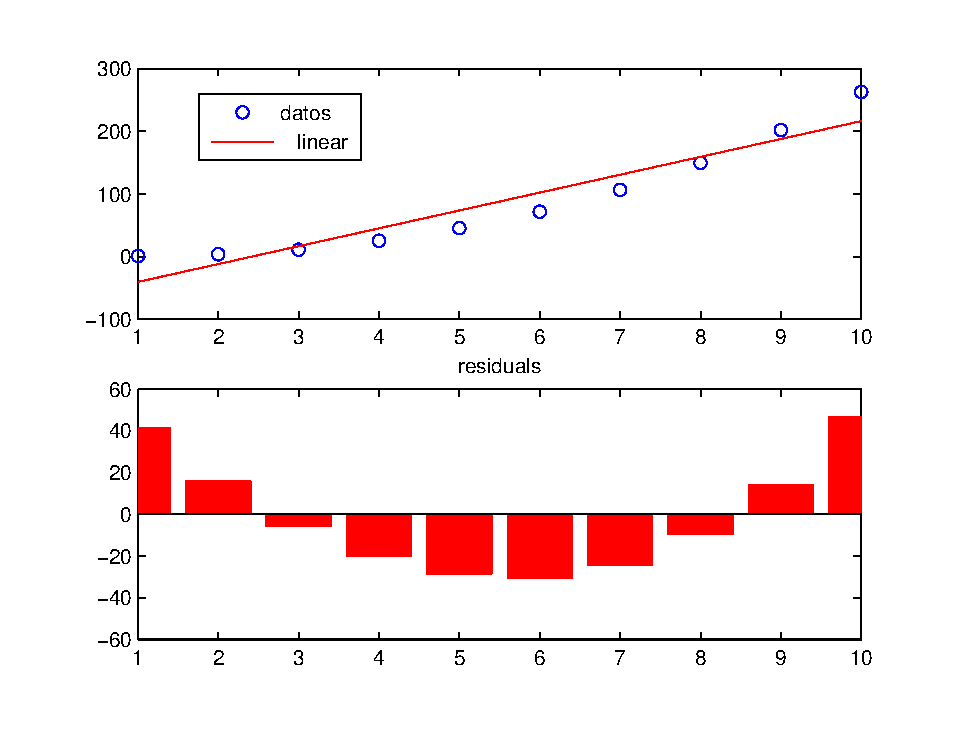
\includegraphics[width=6.5cm]{residuos1.eps}} \qquad 
\subfigure[Parabola de mínimos cuadrados y residuos obtenidos  \label{fig:residuos2}]{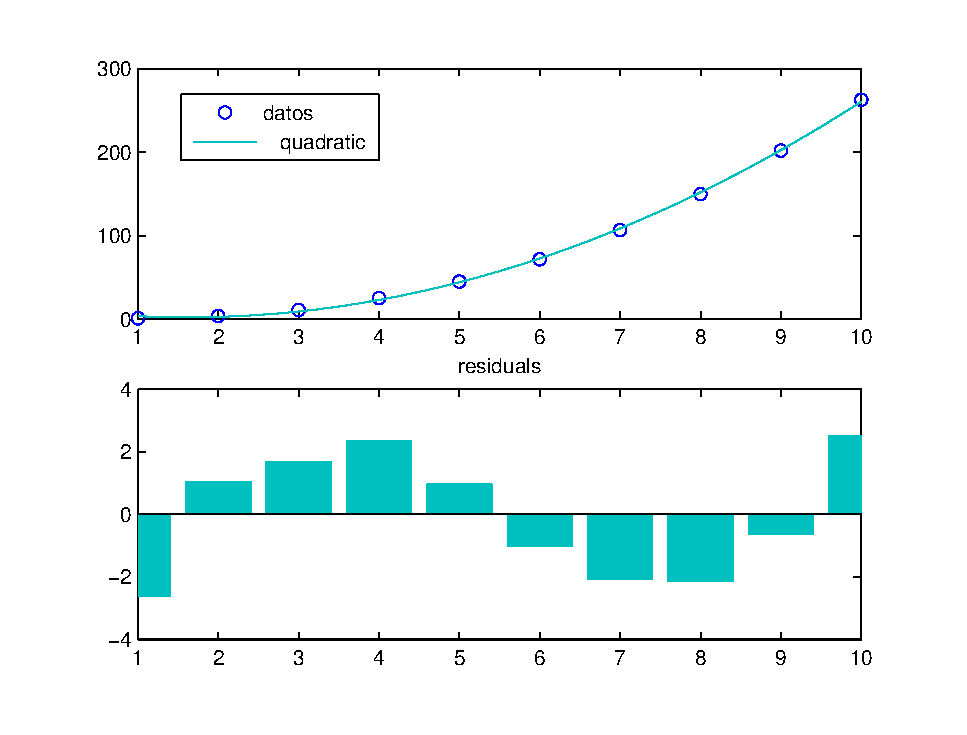
\includegraphics[width=6.5cm]{residuos2.eps}}\\
\subfigure[polinomio de tercer grado  de mínimos cuadrados y residuos obtenidos \label{fig:residuos3}]{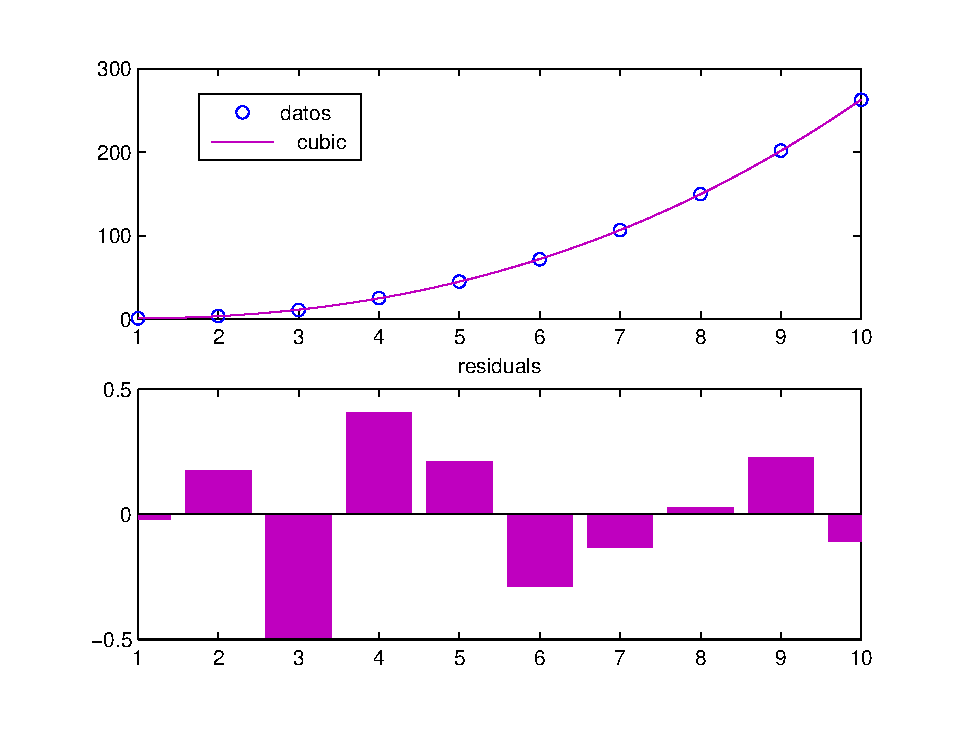
\includegraphics[width=6.5cm]{residuos3.eps}} \qquad 
\subfigure[polinomio de cuarto grado  de mínimos cuadrados y residuos obtenidos  \label{fig:residuos4}]{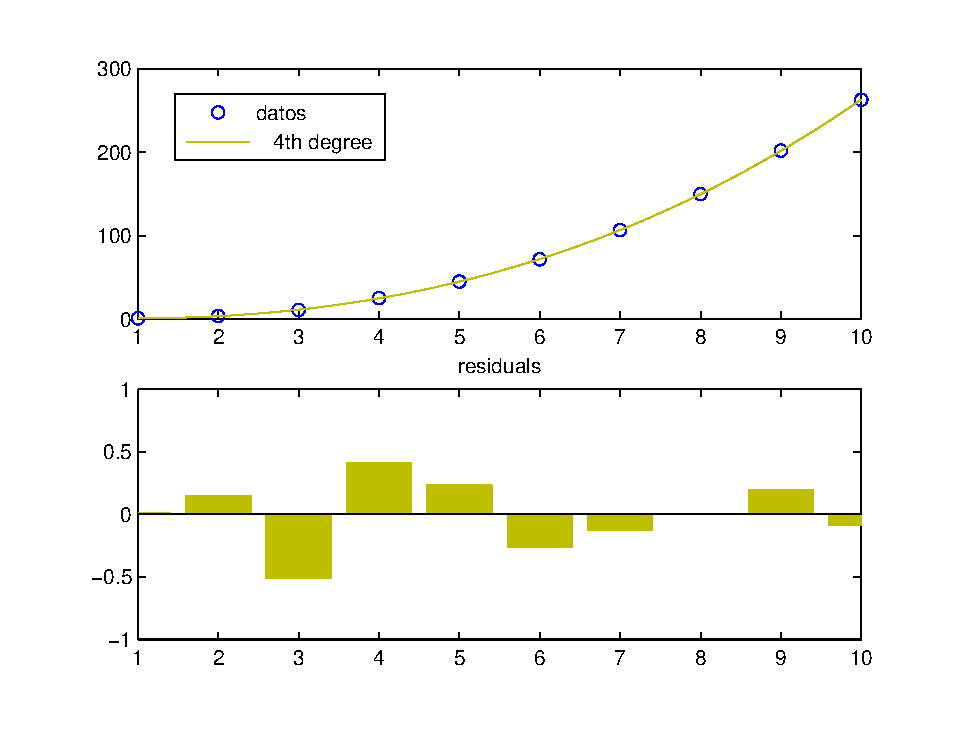
\includegraphics[width=6.5cm]{residuos4.eps}}
\caption{Comparación entre los residuos obtenidos para los ajustes de mínimos cuadrados de un conjunto de datos empleando polinomios de grados 1 a 4.} 
\label{fig:residuos}
\end{figure}
\begin{paracol}{2} 
\section{Curvas de Bézier}\index{Bézier}\index{Curvas de Bézier}
Las curvas de Bézier permiten unir puntos mediante curvas de forma arbitraria.  Una curva de Bézier viene definida por un conjunto de $n+1$ puntos, $\left\lbrace\vec{p}_0, \vec{p}_2, \cdots, \vec{p}_n\right\rbrace$, que reciben el nombre de puntos de control. El orden en que se presentan los puntos de control es importante para la definición de la curva de Bézier correspondiente. Ésta pasa siempre por los puntos $\vec{p_0}$ y $\vec{p_n}$. El resto de los puntos de control permiten dar forma a la curva, que tiene siempre la propiedad de ser tangente en el punto $\vec{p}_0$ a la recta que une $\vec{p}_0$ con $\vec{p}_1$ y tangente en el punto $\vec{p}_n$ a la recta que une $\vec{p}_{n-1}$ con $\vec{p}_n$.

Para definir la curva, se asocia a cada punto de control $\vec{p}_i$ una función conocida con el nombre de función de fusión. En el caso de las curvas de Bézier, las funciones de fusión empleadas son los polinomios de Bernstein, \index{Polinomios de Bernstein}
\end{paracol}
\begin{equation*}
B_i^n (t)=\binom{n}{i}\left(1-t\right)^{n-i}t^i, \quad i = 0, 1, \dots, n
\end{equation*}
\begin{paracol}{2}
El grado de los polinomios de Bernstein empleados está asociado al número de puntos de control; para un conjunto de $n+1$ puntos, los polinomios empleados son de grado $n$. La variable $t$ es un parámetro que varía entre $0$ y $1$.

La ecuación de la curva de Bézier que pasa por un conjunto de $n+1$ puntos de control, $\left\lbrace\vec{p}_0, \vec{p}_2, \cdots, \vec{p}_n\right\rbrace$, se define a partir de los polinomios de Bernstein como,
\end{paracol}
\begin{equation*}
\vec{p}(t) = \sum_{i = 0}^n B_i^n(t) \cdot \vec{p}_i = \sum_{i = 0}^n \binom{n}{i}\left(1-t\right)^{n-i}t^i  \cdot \vec{p}_i
\end{equation*}
\begin{paracol}{2}
La expresión anterior da como resultado $\vec{p}_0$ si hacemos $t = 0$ y $\vec{p}_n$ si hacemos $t = 1$. para los valores comprendidos entre $t=0$ y $t=1$, los puntos $\vec{p}(t)$  trazarán una curva entre $\vec{p}_0$  y $\vec{p}_n$.

Veamos un ejemplo sencillo. Supongamos que queremos unir los puntos $\vec{p}_0 = (0,1)$ y $\vec{p}_n = (3,1)$ mediante curvas de Bézier. Si no añadimos ningún punto más de control, $\lbrace\vec{p}_0 = (0,1), \vec{p}_1 = (3,1)\rbrace$, el polinomio de Bézier que obtendremos será una recta que unirá los dos puntos,
\end{paracol}
\begin{equation*}
\vec{p}(t) = \binom{1}{0}\left(1-t\right)^{1}t^0  \cdot (0,1) +  \binom{1}{1}\left(1-t\right)^{0}t^1  \cdot (3,1) = \left(1-t\right)  \cdot (0,1) + t\cdot (3,1)
\end{equation*} 
\begin{paracol}{2}
Si separamos las componentes $x$ e $y$ del vector $\vec{p}(t)$,
\end{paracol}

\begin{align*}
x &= 3t\\
y &= 1
\end{align*}
\begin{paracol}{2}
Se trata de la ecuación del segmento horizontal que une los puntos $\vec{p}_0 = (0,1)$ y $\vec{p}_n = (3,1)$ 

Si añadimos un punto más de control, por ejemplo:  $\vec{p}_1 = (1,2) \rightarrow \lbrace\vec{p}_0 = (0,1), \vec{p}_1 = (1,2), \vec{p}_2 = (3,1)\rbrace$,  la curva resultante será ahora un segmento de un polinomio de segundo grado en la variable $t$,
\end{paracol}
\begin{align*}
\vec{p}(t) &= \binom{2}{0}\left(1-t\right)^{2}t^0  \cdot (0,1) +  \binom{2}{1}\left(1-t\right)t \cdot (1,2) + \binom{2}{2}\left(1-t\right)^{0}t^2  \cdot (3,1) =\\
&= \left(1-t\right)^{2} \cdot (0,1) + 2 \left(1-t\right)t \cdot (1,2) + t^2  \cdot (3,1) 
\end{align*} 
\begin{paracol}{2}
Según vamos aumentando el número de los puntos de control, iremos empleando polinomios de mayor grado. El segmento de polinomio empleado en cada caso para unir los puntos de control inicial y final variará dependiendo de los puntos de control intermedios empleados.

La figura \ref{fig:bezier} muestra un ejemplo en el que se han construido varias curvas de Bézier sobre los mismos puntos de paso inicial y final. Es fácil observar cómo la forma de la curva depende del número y la posición de los puntos de control. Si unimos éstos por orden mediante segmentos rectos, obtenemos un polígono que recibe el nombre de polígono de control. En la figura \ref{fig:bezier} se han representado los polígonos de control mediante líneas de puntos.

El siguiente código permite calcular y dibujar una curva de Bézier a partir de sus puntos de control.
\end{paracol}
%\begin{lstlisting}
%function ber = bezier(p,res)
%% estas funcion pinta la curva de Bezier correspondiente a los puntos de 
%% control p. 
%% p debe ser una matriz de dimension n*2 donde n es el número de puntos de 
%% control empleados La primera columna contiene las coordenadas x 
%% y la segunda las coordenas y.
%% El codigo sigue directamente la definicion de los polinomios de Bernstain
%% por tanto, NO es un codigo optimo. Calcula varias veces las mismas
%% cantidades.
%% Los coeficientes binomiales de los polinomios de Berstein se 
%% pueden calcular directamente con el comando de matlab nchoosek. Sin 
%% enbargo, en el programa se han calculado a partir de la definicion:
%%  n!/((n-k)!k!)
%% la variable de entrada res nos da el paso que empleará el parámatro t
%% para calcular y dibujar el polinomio
%
%t = 0:res:1;
%ber = zeros(2,length(t));
%% calculamos un vector de coeficientes para los polinomios.
%
%% coeficientes para la coordenada x.
%
%n = size(p,1)-1;
%num = factorial(n);
%for i = 0:n    
%    f=num/factorial(i)/factorial(n-i);
%    ber(1,:) = ber(1,:) + f*p(i+1,1)*(1-t).^(n-i).*t.^i;
%    ber(2,:) = ber(2,:) + f*p(i+1,2)*(1-t).^(n-i).*t.^i;
%end
%plot(p(:,1),p(:,2),'or')
%hold on
%plot(p(:,1),p(:,2),'r')
%plot(ber(1,:),ber(2,:))
%\end{lstlisting}

\begin{figure}[h]
\centering
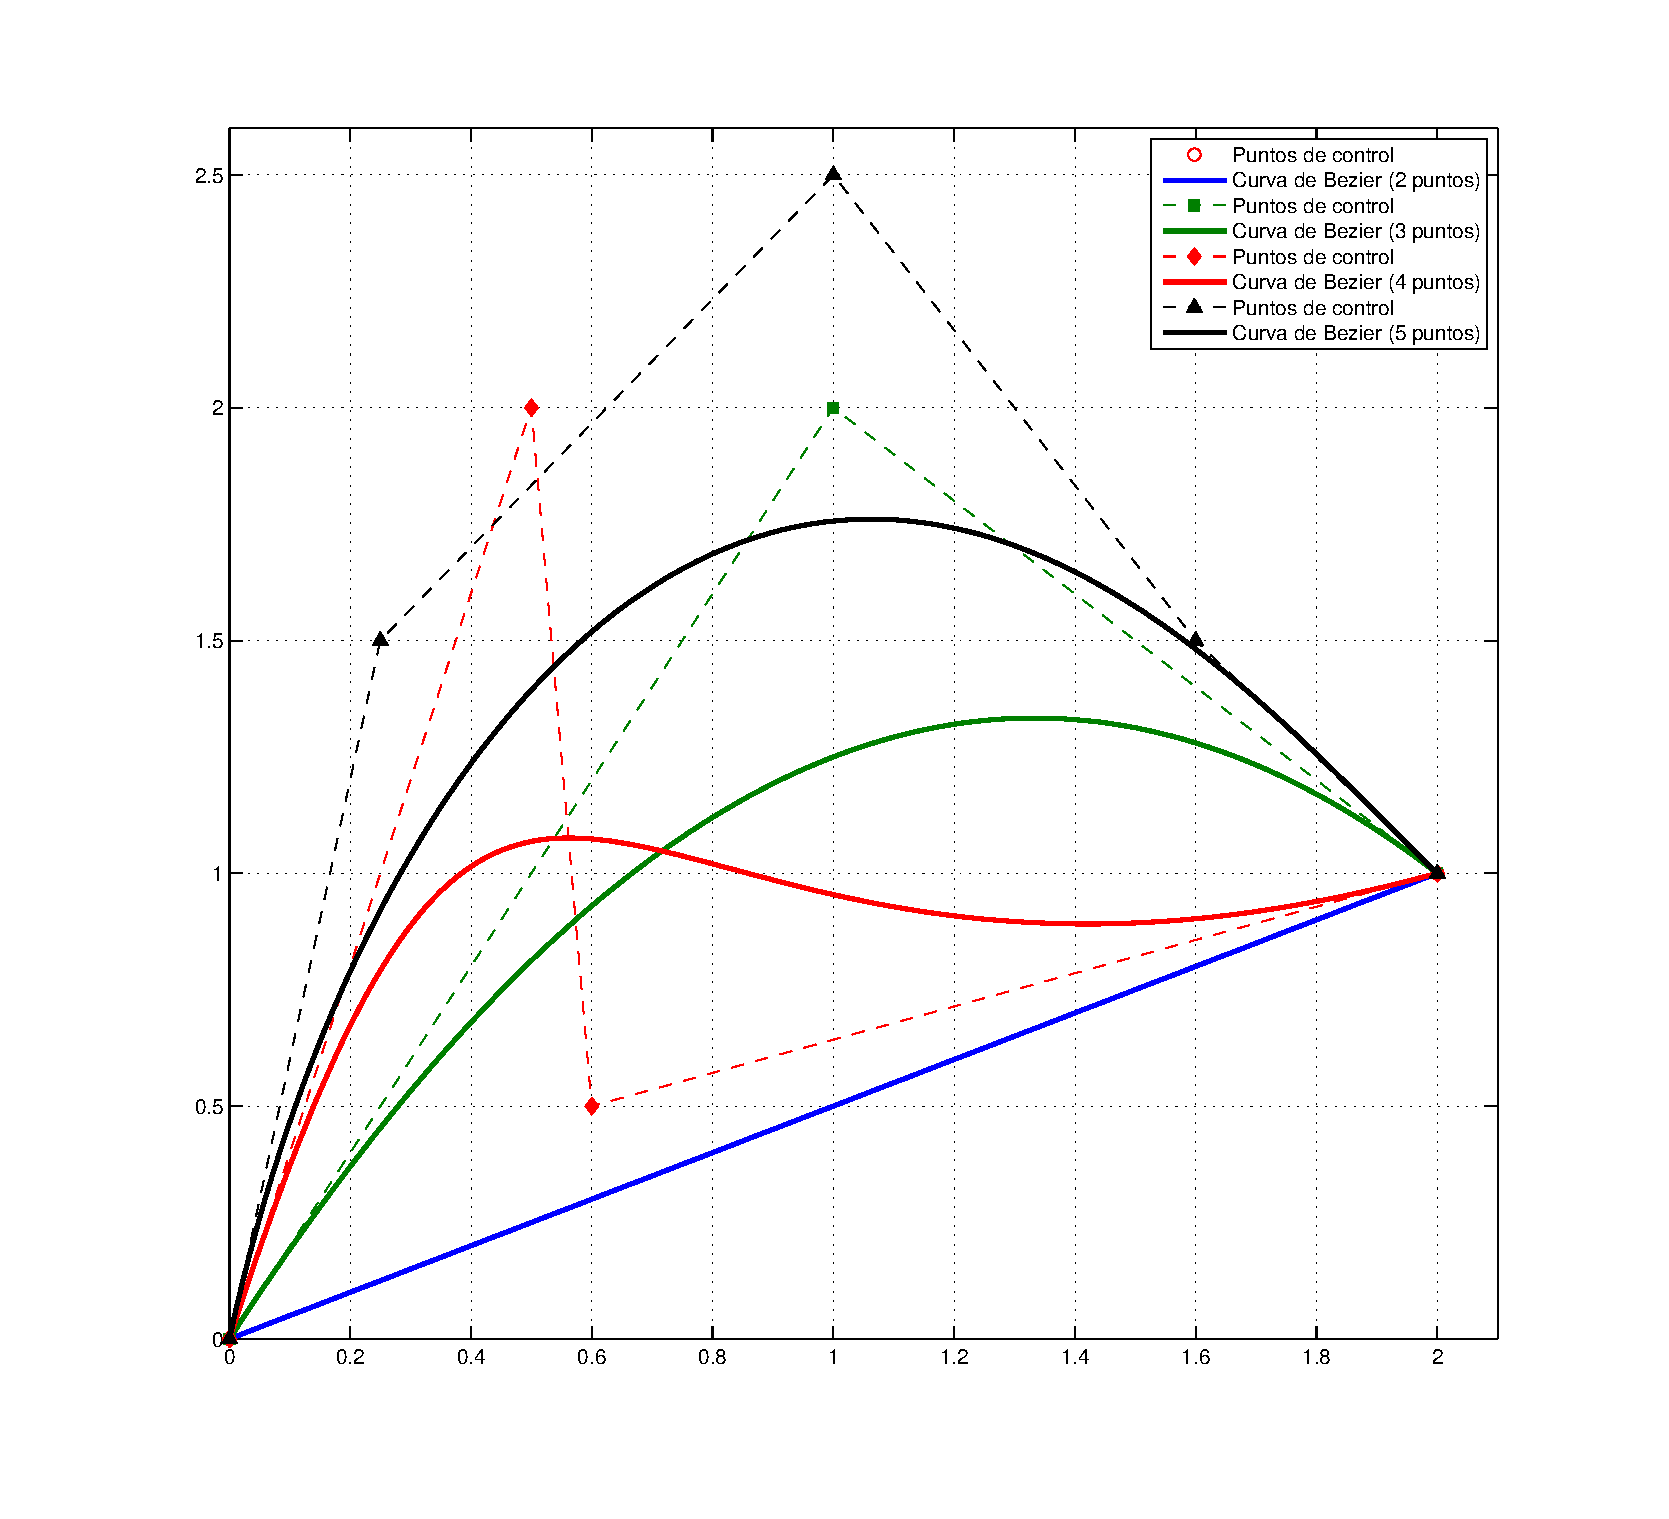
\includegraphics[width=10cm]{bezier.eps} 
\caption{Curvas de Bézier trazadas entre los puntos $P_0 = (0,0)$ y $P_n = (2,1)$, variando el número y posición de los puntos de control.} 
\label{fig:bezier}
\end{figure}
\begin{paracol}{2}
\paragraph{Curvas equivalentes de grado superior.} Dada una curva de Bézier, representada por un polinomio de Bernstein de grado $n$, es posible encontrar polinomios de grado superior que representan la misma curva de Bézier. Lógicamente esto supone un aumento del número de puntos de control.

Supongamos que tenemos una curva de Bézier con cuatro puntos de control,
\end{paracol}
\begin{equation*}
\vec{p}(t) = \vec{p}_0B_0^3(t) + \vec{p}_1B_1^3(t) + \vec{p}_2B_2^3(t) + \vec{p}_3B_3^3(t)
\end{equation*}
\begin{paracol}{2}
Si multiplicamos este polinomio por $ t + (1 -t) \equiv 1$ El polinomio no varía y por tanto representa la misma curva de Bézier. Sin embargo, tendríamos ahora un polinomio un grado superior al inicial.  Si después de la multiplicación agrupamos términos de la forma $(1-t)^{n-1}t^i$, Podríamos obtener el valor de los nuevos puntos de control,
\end{paracol}
\begin{align*}
\vec{p}_0^+&= \vec{p}_0\\
\vec{p}_1^+&= \frac{1}{4}\vec{p}_0 + \frac{3}{4}\vec{p}_1\\
\vec{p}_2^+&= \frac{2}{4}\vec{p}_2 + \frac{2}{4}\vec{p}_3\\
\vec{p}_3^+&= \frac{3}{4}\vec{p}_2 + \frac{1}{4}\vec{p}_3\\
\vec{p}_4^+&= \vec{p}_3\\
\end{align*}
\begin{paracol}{2}
y, en general, los puntos de control de la curva de Bézier de grado $n+1$ equivalente  a una dada de grado $n$ puede obtenerse como,
\end{paracol}
\begin{equation*}
\vec{p}_i^+ = \alpha_i\vec{p}_{i-1} + (1-\alpha_i)\vec{p}_i, \qquad \alpha_i =\frac{i}{n+1}
\end{equation*}
\begin{paracol}{2}
Mediante la ecuación anterior, es posible obtener iterativamente los puntos de control de la curva de Bézier equivalente a una dada de cualquier grado. Una propiedad interesante es que según aumentamos el número de puntos de control empleados, estos y el polígono de control correspondiente, van convergiendo a la curva de Bézier. 

La figura \ref{fig:bzgrad} muestra un ejemplo para una curva de Bézier construida a partir de tres puntos de control. Es fácil ver cómo a pesar de aumentar el número de puntos de control, la curva resultante es siempre la misma.  También es fácil ver en la figura (\ref{fig:bz4}) la convergencia de los polígonos de control hacia la curva.
\end{paracol}
\begin{figure}[h]
\centering
\subfigure[Curva original (3 puntos) \label{fig:bz1}]{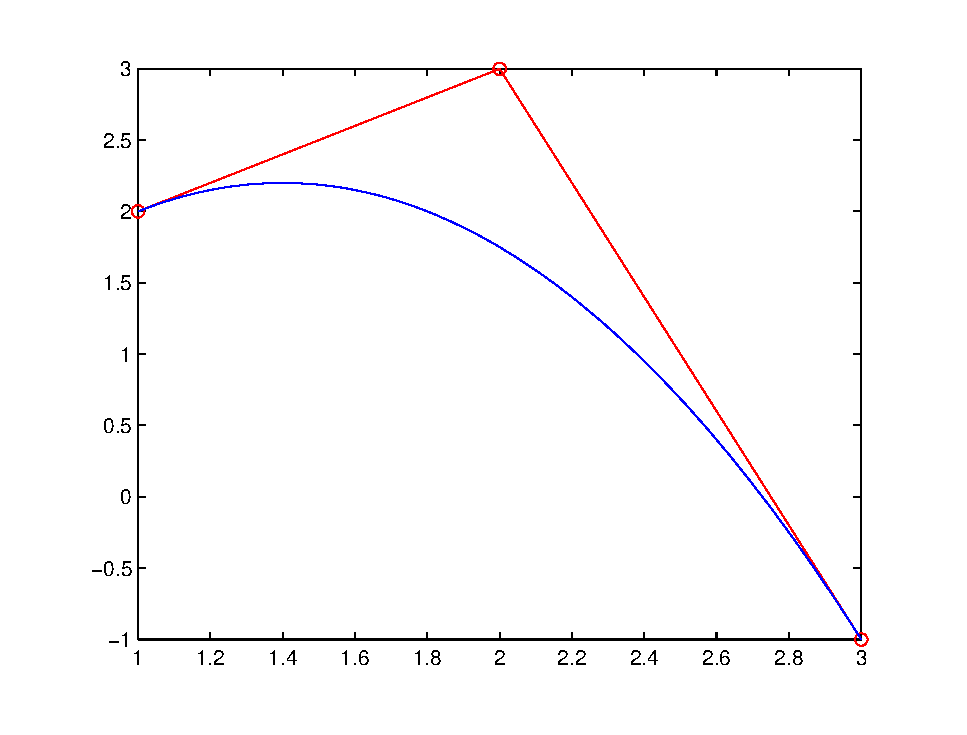
\includegraphics[width=6.8cm]{bezier3p.eps}} \qquad 
\subfigure[Curvas equivalentes de 4 a 6 puntos  \label{fig:bz2}]{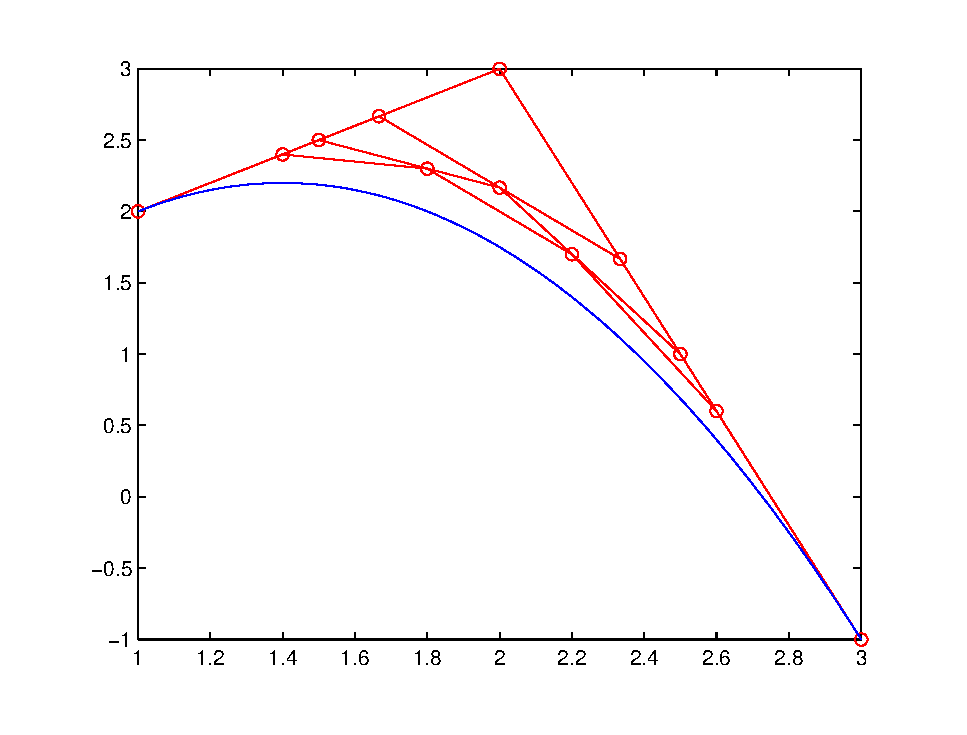
\includegraphics[width=6.8cm]{bezier6p.eps}}\\
\subfigure[Curvas equivalentes de 4 a 12 puntos  \label{fig:bz3}]{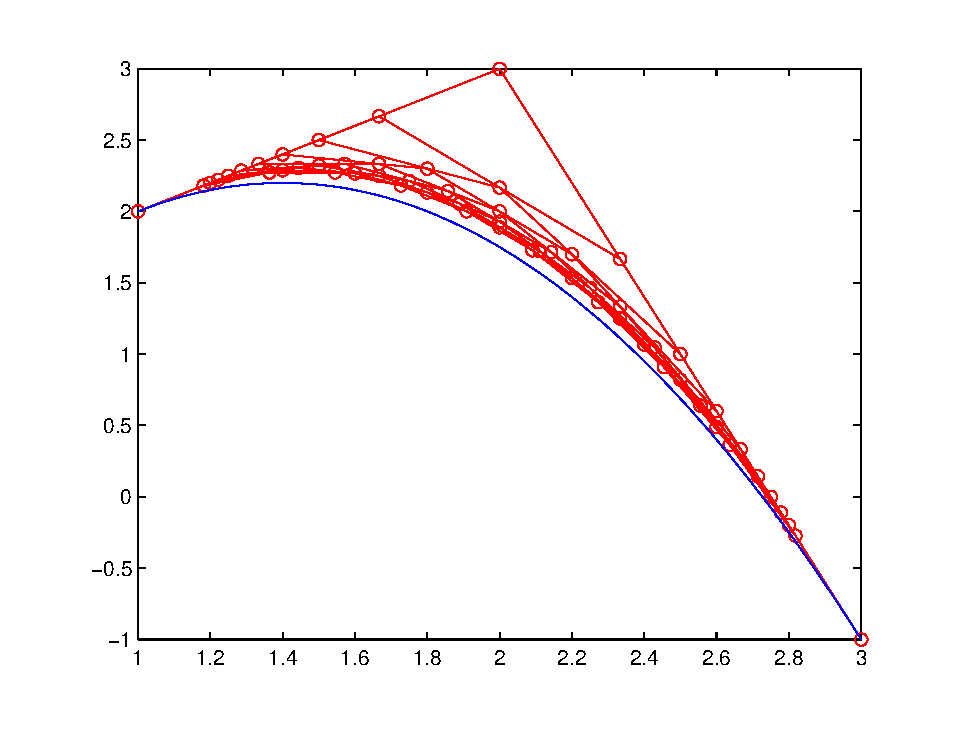
\includegraphics[width=6.8cm]{bezier12p.eps}} \qquad 
\subfigure[Curvas equivalentes de de 4 a 30 puntos  \label{fig:bz4}]{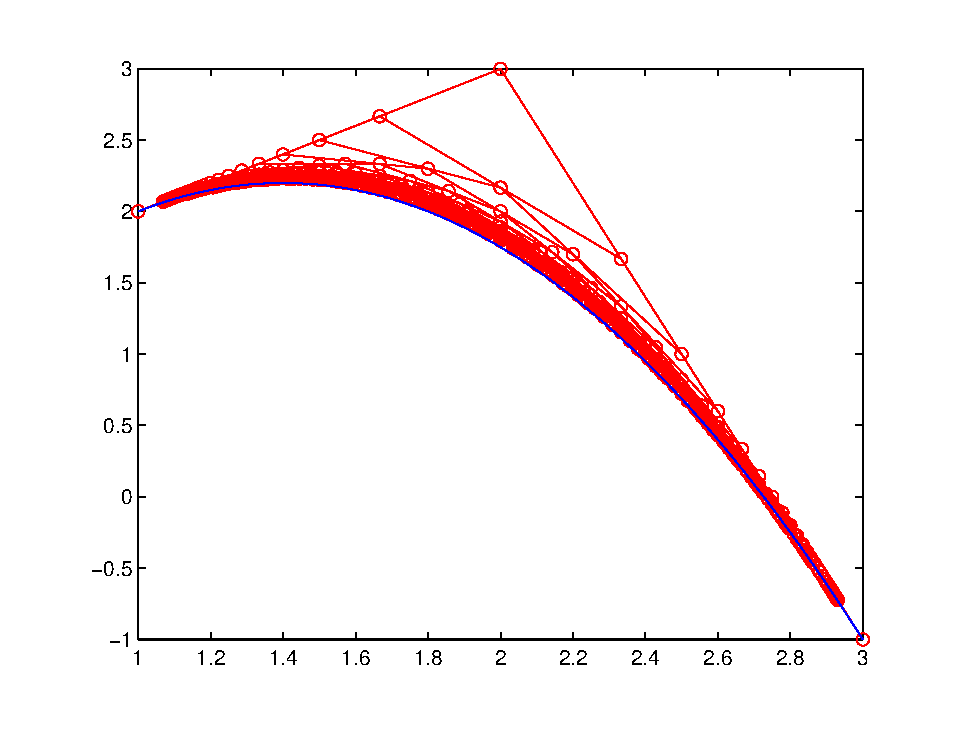
\includegraphics[width=6.8cm]{bezier30p.eps}}
\caption{Curvas de Bézier equivalentes, construidas a partir de una curva con tres puntos de control} 
\label{fig:bzgrad}
\end{figure}
\begin{paracol}{2}
El siguiente código permite calcular la curva equivalente de Bézier a una dada, para cualquier número de puntos de control que se desee. \index{Curvas de Bézier equivalentes}
\end{paracol}
%\begin{lstlisting}
%function  pp = bzeq(p,n)
%% Esta funcion calcula los puntos de control de una curva de Bezier
%% equivalente de grado superior. p es matriz de tamaño mx2 que contiene 
%% los puntos de control originales. n es el número de puntos de paso de 
%% la nueva curva de Bezier equivalente. n tiene que ser mayor que m.
%% pp contiene los n puntos de control de la curva de Bézier resultante.
%
%% Construimos un vector  con una fila mas para guardar un nuevo elemento
%c = size(p,1);
%% La siguiente linea sirve solo para ir pintando los resultados y ver 
%%que  efectivamente todos los polinomios dan la misma curva de Bezier 
%%  (si se tiene la funcion bezier).
%bezier(p,0.01);
%if c == n
%    pp = p;
%    return
%else
%    p = [p;zeros(1,2)];
%    pp = p;
%    for i = 2 : c+1
%        pp(i,:) = p(i-1,:)*(i-1)/(c) + (1 -(i-1)/(c))*p(i,:);
%        
%    end
%    % llamamos a la funcion recursivamente hasta tener n puntos de 
%    % control el grado del polinomio sera n-1...
%    pp = bzeq(pp,n);
%end
%\end{lstlisting}
\begin{paracol}{2}
\paragraph{Derivadas.} Las derivadas de una curva de Bézier con respecto al parámetro $t$ son particularmente fáciles de obtener a partir de los puntos de control. Si tenemos una curva de Bézier de grado $n$, definida mediante puntos de control $\vec{p}_i$ su derivada primera con respecto a $t$ será una curva de Bézier de grado $n-1$ Cuyos puntos de control $\vec{d}_i$  puede obtenerse como:
\end{paracol}
\begin{equation*}
\vec{d_i} = n\left(\vec{p_{i+1}} -\vec{p_i}\right)
\end{equation*}
\begin{paracol}{2}
La nueva curva de Bézier obtenida de este modo, es una hodógrafa; representa el extremo de un vector tangente en cada punto a la curva de Bézier original  y guarda una relación directa con la velocidad a la que se recorrería dicha curva. \index{hodógrafa}

La figura \ref{fig:bzc}, muestra una curva de Bézier sobre la que se ha trazado el vector derivada para algunos puntos. La figura \ref{fig:bzd} muestra la hodógrafa correspondiente y de nuevo los mismos vectores derivada de la figura \ref{fig:bzc}

El siguiente código muestra como calcular los puntos de control de la derivada de una curva de Bézier.
\end{paracol}
%\begin{lstlisting}
%function d = dbez(p)
% esta función obtiene los puntos de control de la derivada con 
% respecto al parametro de una curva de bezier cuyos puntos de  
% control están contenidos la matriz p. p de be ser una matriz de 
% nx2 donde n es el número de puntos de control.
%grado = size(p,1) -1
%d = zeros(grado,2)
%for i = 1:grado
%    d(i,:) = (grado-1)*(p(i+1,:)-p(i,:))
%end
% Codigo añadido para dibujar y analizar los resultados
% pintamos la hodografa
%v = bezier(d,0.01)
% le añadimos algunos vectores para que se vea que tocan la hodografa
% hold on
% compass(v(1,1:10:size(v,2)),v(2,1:10:size(v,2)))
% figure
%% las pintamos además como vectores tangentes a la curva original
%x = bezier(p,0.01)
%hold on
%quiver(x(1,1:10:size(v,2)),x(2,1:10:size(v,2)),v(1,1:10:size(v,2))...
%    ,v(2,1:10:size(v,2)))
%\end{lstlisting}

\begin{figure}
\centering
\subfigure[Curva de Bézier (4 puntos) \label{fig:bzc}]{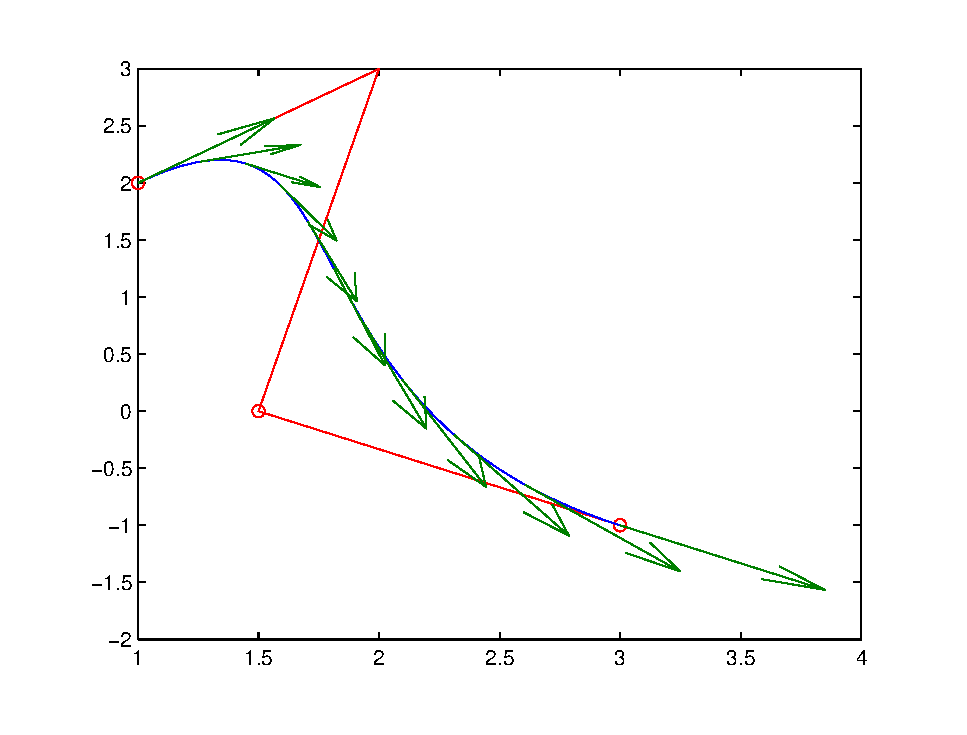
\includegraphics[width=7cm]{bezierder.eps}} \qquad 
\subfigure[Derivada (hodógrafa)  \label{fig:bzd}]{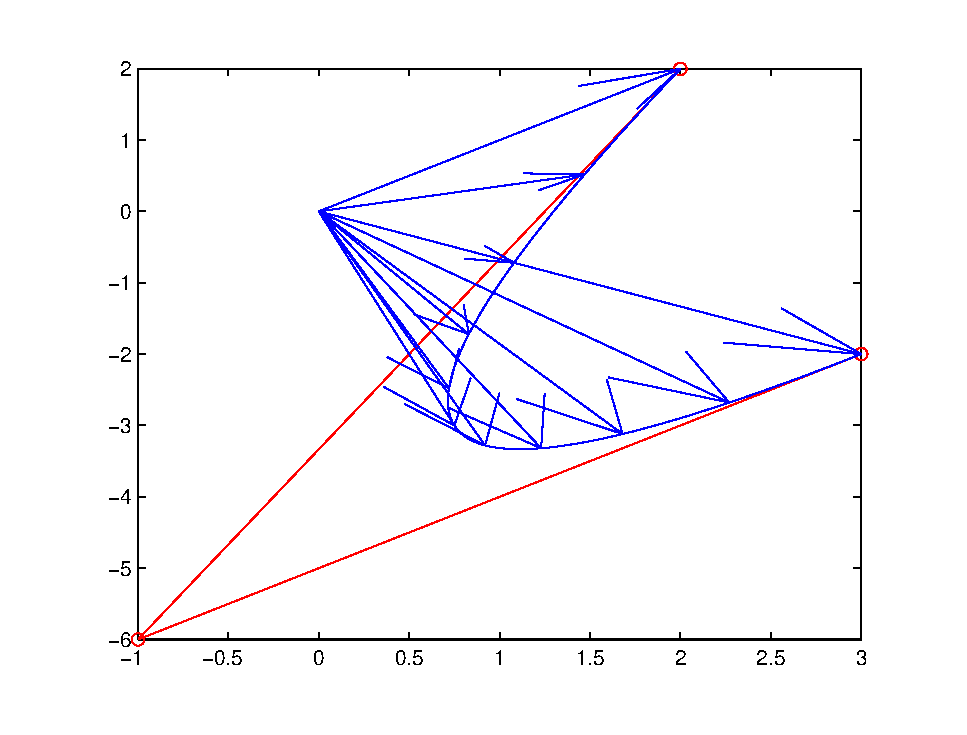
\includegraphics[width=7cm]{bezierhodg.eps}}
\caption{Curva de Bézier y su derivada con respecto al parámetro del polinomio de Bernstein que la define: $t \in [0,1]$} 
\label{fig:bzder}
\end{figure} 
\begin{paracol}{2}
\paragraph{Interpolación con curvas de Bézier} Podemos emplear curvas de Bézier para interpolar un conjunto de puntos $\lbrace \vec{p}_0, \cdots  \vec{p}_m\rbrace$. Si empleamos un curva para interpolar cada par de puntos, $\vec{p}_i, \vec{p}_{i+1}, \qquad i =1, \cdots m-1$ tenemos asegurada la continuidad en los puntos interpolados puesto que las curvas tienen que pasar por ellos. Como en el caso de la interpolación mediante splines, podemos imponer continuidad en las derivadas para conseguir una curva de interpolación suave. En el caso de las curvas de Bézier esto es particularmente simple. Si llamamos $B$ a la curva de Bézier de grado $n$ construida entre los puntos $\vec{p}_{i-1}, \vec{p}_{i}$  con puntos de control, $\vec{p}_{i-1}, b_1, \vec{b}_2,\cdots, \vec{b}_{n-1},\vec{p}_{i}$. Y  $C$ a la curva de Bézier de grado $s$ construida entre los puntos $\vec{p}_{i}, \vec{p}_{i+1}$  con puntos de control, $\vec{p}_{i}, \vec{c}_1, \vec{c}_2,\cdots, \vec{c}_{s-1},\vec{p}_{i+1}$. Para asegurar la continuidad en la primera derivada en el punto $\vec{p_i}$ basta imponer,
\end{paracol}
\begin{equation*}
n\cdot\left(\vec{p}_i-\vec{b}_{n-1}\right) = s\cdot\left(\vec{c}_1-\vec{p}_i\right)
\end{equation*}
\begin{paracol}{2}
Esta condición impone una relación entre el penúltimo punto de control de la curva $B$ y el segundo punto de control de la curva $C$. Pero deja completa libertad sobre el resto de los puntos de control elegidos para construir las curvas.

Podemos, por ejemplo, elegir libremente todos los puntos de control de la curva $B$ y obtener a partir de ella el punto $\vec{c}_1$,
\end{paracol}
\begin{equation*}
\vec{c}_1 = \frac{n+s}{s}\vec{p}_i - \frac{n}{s}\vec{b}_{n-1}
\end{equation*}

\begin{figure}[h]
\centering
\subfigure[Interpolación mediante curvas de Bézier de 3 puntos) \label{fig:ibz}]{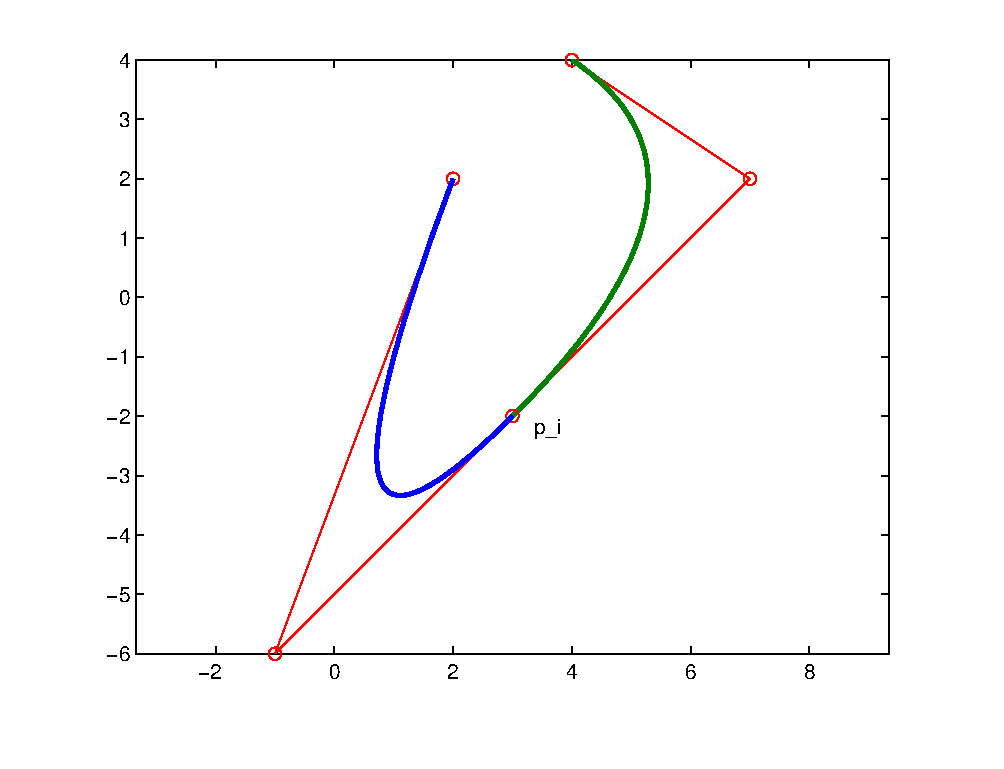
\includegraphics[width=7cm]{bezierint.eps}} \qquad 
\subfigure[Interpolación mediante curvas de Bézier de 3 y 4 puntos  \label{fig:ibz2}]{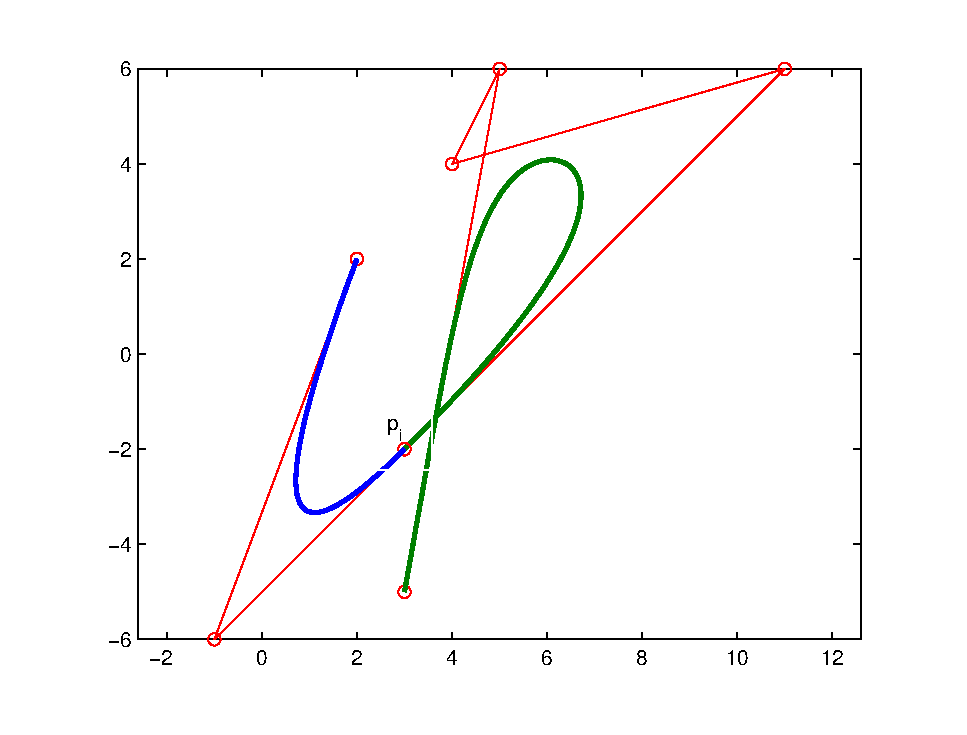
\includegraphics[width=7cm]{bezierint2.eps}}
\caption{Interpolación de tres puntos mediante dos curvas de Bézier} 
\label{fig:ibz3}
\end{figure}
 
\begin{paracol}{2}
La figura \ref{fig:ibz3} muestra un ejemplo de interpolación en la que se ha aplicado la condición de continuidad en la derivada que acabamos de describir.
\end{paracol}
\section{ejercicios}
\begin{enumerate}
\item Carga en Matlab los datos del fichero \texttt{datos.txt}\footnote{disponible en \url{https://github.com/UCM-237/LCC/tree/master/datos}} y realiza las siguientes tareas:
\begin{enumerate}
\item \label{ej1a} Crea una función que a partir de dos vectores de datos $x,y$ de igual longitud $n+1$, calcula la matriz de Vandermonde necesaria   para obtener el polinomio de interpolación asociado a los puntos. Empleando la primera columna de datos contenida en \texttt{datos.txt} como datos $x$ y la segunda como datos $y$, genera el polinomio de interpolación,
\begin{equation*}
p(x)=a_0+a_1x+a_2x^2+\cdots+a_nx^n
\end{equation*}

Calcula el valor que toma el polinomio de interpolación en 100 puntos equiespaciados entre los valores $x_0$ y $x_{n}$ de los datos del fichero. Dibuja en una misma gráfica los resultados obtenidos, empleando una línea continua, y los valores del fichero, mediante puntos separados empleando el símbolo que prefieras. Comprueba que el polinomio pasa por los puntos contenidos en el fichero.

\item Reproduce en matlab la función 'Lagrange' de la sección \ref{sec:lagranje} para calcular el polinomio interpolador de Lagrange. Emplea la función que acabas de crear para recalcular los valores del polinomio de interpolación realizado en el ejercicio anterior y comprueba que los resultados obtenidos son los mismos que empleando la matriz de Vandermonde.

\item A partir de los ejemplos de la sección  sección \ref{sec:difdiv}, crea un programa que calcule los coeficientes del polinomio interpolador de diferencias divididas a partir de dos vectores de datos  $x,y$ de igual longitud $n+1$ y un segundo programa que calcule el valor del polinomio en un punto cualquiera a partir de los coeficientes obtenidos con el primer programa. Vuelve a calcular, empelando ahora el polinomio de diferencias dividas, los valores del polinomio de interpolación sobre los mismos datos empleados en los ejercicios anteriores y comprueba que da los mismos resultados.

\item Por último, crea una función que calcule el polinomio de interpolación de Newton-Gregory (sección \ref{sec:newgre}). ¿Es posible usarlos para interpolar los datos del archivo \texttt{datos.txt}? Si la respuesta el afirmativa, repite el cálculo del polinomio de interpolación, empleando Newton-Gregory y comprueba si coincide con lo obtenido en los ejercicios anteriores.

\item Usa el comando \texttt{help} para conocer los distintos métodos de interpolación por intervalos disponibles  para la función \texttt{interp1}. Empleando de nuevo los datos del fichero \texttt{datos.txt}, obtén el resultado de interpolar los valores en 100 puntos equiespaciados entre los valores $x_0$ y $x_{n}$ de los datos del fichero mediante \texttt{interp1}.  Emplea para ello los métodos \texttt{'nearest','linear'} y \texttt{'spline'}. Dibuja los resultados en la misma gráfica empleada en el ejercicio  \ref{ej1a})
\end{enumerate}
\item Construye a partir del código de ejemplo de la sección \ref{sec:mc}, una función que calcule el polinomio de grado $n$ que ajusta por mínimos cuadrados un conjunto de pares de datos datos $(x, y)$. Pruébalo sobre los datos del fichero \texttt{datos.txt}, sin emplear pesos. Compara los coeficientes del polinomio obtenido con los que se obtienen empleando el comando \texttt{polyfit} de Matlab. ¿Qué conclusión sacas?

\item Añade el código necesario al programa anterior para que, una vez obtenidos los coeficientes del polinomio de mínimos cuadrados, la función calcule y devuelva un vector $r$ con los valores de los residuos, $r = y -p(x)$, donde $x$ e $y$ son los vectores del conjunto de datos para los que se ha obtenido el polinomio de mínimos cuadrados y $p$ los valores obtenidos aplicando el polinomio a los valores $x$ de la colección de datos.
\end{enumerate}


\section{Test del curso 2020/21}

% El archivo con los datos lo puedes encontrar en
%\url{}

\noindent \textbf{Problema 1}. Una cuerda de escalada aumenta su longitud cuando está sometida a una tensión estacionaria en uno de sus extremos. En particular, el aumento de longitud sigue la siguiente ley
\begin{equation}\label{eq:0}
T = b\tanh(ax),
\end{equation}
donde $T \in \mathbb{R}^+$ es la tensión aplicada en Newtons, $x \in \mathbb{R}^+$ es la elongación de la cuerda en metros y $a, b \ \in \mathbb{R}^+$ son parámetros constantes que dependen de las características de la cuerda.

En función del comportamiento físico de la cuerda, podemos distinguir tres regímenes:

\begin{itemize}
	\item \emph{Comportamiento elástico}: Se dice que el comportamiento de la cuerda es elástico si al desaparecer la tensión la cuerda recupera su longitud original. Esto se cumple para tensiones estacionarias pequeñas, y las elongaciones están acotadas por un valor positivo $x_{le}$, esto es, $0 \le x \le x_{le}$. En régimen elástico, la ecuación (\ref{eq:0}) puede aproximarse por la siguiente expresión
\begin{equation}\label{eq:1}
T = \kappa x - \gamma x^3,
\end{equation}
donde $\kappa,\gamma \in \mathbb{R}^+$ son también constantes.

\item \emph{Comportamiento plástico}: Se dice que el comportamiento de la cuerda es plástico si al desaparecer la tensión la cuerda se deforma y no recupera su longitud original. Esto ocurre para tensiones medias, y la elongación alcanzada en este régimen está también acotada por $x_{le} < x \le x_{max}$.

\item \emph{Rotura}: Para tensiones grandes la cuerda no admite elongaciones mayores que $x_{max}$ y se rompe.

\end{itemize}

La fábrica de cuerdas de escalada \textit{Pa'bennos Matao S.L.} ha realizado un estudio sobre un nuevo modelo de cuerda. En dicho estudio se fijó un extremo de la cuerda a una mesa abatible suficientemente grande (que hará la función de un plano inclinado), y se ató el otro extremo de la cuerda a una pesa. De manera secuencial se fue incrementando el ángulo formado por la mesa con la horizontal. En particular, se empezó con cero grados y aumentando el ángulo hasta que finalmente la cuerda alcanzó $x_{max}$ y se rompió. 

Del estudio se pudo registrar la elongación sufrida por la cuerda por los distintos $i\in\{1,\dots,52\}$ ángulos de inclinación. Estos datos están en el archivo:  \texttt{cuerda.txt}\footnote{disponible en \url{https://github.com/UCM-237/LCC/tree/master/datos}}, en donde:
\begin{itemize}
	\item La primera columna corresponde a los ángulos $\theta_i$ medidos en radianes.
	\item La segunda columna corresponde a las elongaciones $x_i$ medidas en metros.
\end{itemize}

\begin{enumerate}
\item (\textbf{1 punto}) Estima el valor de la elongación $x_{max}$ para el cual se produce la rotura de la cuerda.

\item (\textbf{1 punto}) Obtén la tensión ejercida por la pesa sobre la cuerda para cada ángulo de inclinación $\theta_i$ de la mesa, esto es
\begin{equation} \label{eq:2}
T_i = mg\sin(\theta_i),
\end{equation}
donde $m =1000$ Kg y $g = 9.8$ m/s$^2$. Representa gráficamente los datos: $T_i$ frente a $x_i$.

\item A partir de los pares de datos $T_i$ y $x_i$ podemos estimar la ecuación (\ref{eq:1}).
\begin{enumerate}
\item (\textbf{2 puntos}) Ajusta los datos por mínimos cuadrados a un polinomio de grado tres. Dado que dicha aproximación solo es válida para el régimen de comportamiento elástico, es imprescindible realizar el ajuste del polinomio asignando pesos a cada par de datos. Para dar más valor a las elongaciones pequeñas y menos a las grandes, utiliza la siguiente expresión para definir los pesos
\begin{equation}
\omega_i = e^{-10x_i^2}.
\end{equation}
\item (\textbf{1 punto})  Representa, sobre la gráfica dibujada en el apartado 2a, el polinomio obtenido en el apartado 3a. Según tu criterio, ¿es razonable el ajuste realizado? \\ \textbf{Nota:} Recuerda que el vector de coeficientes, obtenido con el algoritmo de mínimos cuadrados del manual, está ordenado al revés con respecto a lo que esperan las funciones de Matlab. Puedes reordenarlo a mano o con el comando \texttt{flipud(p)}.
\end{enumerate}

\item (\textbf{1 punto})  Los coeficientes de las ecuaciones (\ref{eq:0}) y (\ref{eq:1}) están relacionados por las siguientes expresiones
\begin{equation}
\kappa = b\cdot a, \quad \gamma = \frac{b\cdot a^3}{3}. \nonumber
\end{equation}
		Calcula los valores de $a$ y $b$ a partir de los coeficiente del polinomio obtenido en el apartado 3a. Representa, en la misma gráfica de los apartados anteriores, la función $T(x) = b\tanh(ax)$. Explica, a la vista del gráfico, si los resultados obtenidos son razonables o no. 

\item (\textbf{1 punto}) Calcula el valor de los residuos $r_i = T_i - P_3(x_i)$, donde $P_3(x)$ es el polinomio de grado tres obtenido en el apartado 3a. Si la cota $x_{le}$ para el comportamiento elástico de la cuerda viene definida cuando $r_i \approx 500 N$. Encuentra un valor aproximado para $x_{le}$. \\
\textbf{Nota:} Hay que buscar $x_{le}$ empleando código. No vale dibujar los residuos y estimarlo a vista.
\end{enumerate}

\noindent \textbf{Problema 2.} Dados los siguiente valores de la función $f(x)$:
\begin{equation}
f(0) = 1, \quad f \left(\frac{\pi}{4}\right)= \frac{\sqrt{2}}{2}, \quad f \left(\frac{\pi}{2}\right) = 0, \quad f \left(\frac{3\pi}{4}\right) = -\frac{\sqrt{2}}{2}, \quad f(\pi) = -1 \nonumber
\end{equation}
\begin{enumerate}
\item (\textbf{1.5 puntos}) Utilizando el comando de Matlab correspondiente. Obtener mediante interpolación con splines cúbicos los valores de la función $f(x)$ sobre cien puntos equiespaciados en el intervalo $[0,\pi]$.

\item (\textbf{1.5 puntos}) Dibuja mediante un diagrama de barras los errores cometidos entre los $f(x)$ y la función $\cos(x)$ de Matlab en los mismos puntos del intervalo anterior. Considera que no necesitamos saber más de dos decimales para el cálculo de la función coseno; ¿podríamos utilizar la interpolación para $f(x)$?
\end{enumerate}



